\documentclass[10pt]{article}
\usepackage[margin=0.75in]{geometry}
\usepackage{amsmath,amssymb,booktabs,graphicx,longtable,placeins,float,hyperref}
\hypersetup{hidelinks}
\graphicspath{{figures/}}
\setlength{\emergencystretch}{2em}
\title{Supplementary information\\Cross-fitted selective recovery under controlled multi-sensor corruption}
\author{Riyang Luo}
\date{}
\renewcommand{\thetable}{S\arabic{table}}
\renewcommand{\thefigure}{S\arabic{figure}}
\begin{document}
\maketitle

\section{Algorithm and implementation details}

For every training minibatch, PDRF encodes each available sensor group, computes group logits and bounded scores, and forms normalized weights. One available group is sampled from the training prior. The group receives Gaussian degradation whose scale is determined by a uniformly sampled retention factor. The model then evaluates the degraded view and, when another group remains, the selected-group removal view. The main-text objective combines clean classification, bounded score, boundary, degraded classification, consistency, normalized-weight monotonicity and severity-linked score ranking. All random choices use explicitly recorded seeds.

The RO-PDRF family uses the same architecture and data views. In the formal protocol, the detached clean-view probability vector is the teacher for degraded-view KL distillation; it therefore requires no test label or oracle view selection. RO-PDRF-Lite adds only this recovery term at weight 0.30 to the base PDRF objective and is the primary practical model and software default. RO-PDRF-Full additionally applies clean/degraded multiclass Brier terms, a log interior penalty on both response paths and a smooth one-versus-rest pairwise loss on degraded logits at weights 0.05, 0.005 and 0.10; it is the mechanistic full model. For a minibatch $\mathcal B$, both task losses use the exact class-weighted mean $\sum_{i\in\mathcal B}\omega_{y_i}[-\log p_{iy_i}]/\sum_{i\in\mathcal B}\omega_{y_i}$, evaluated on clean and degraded logits respectively. Consistency, recovery and removal-dependent directional terms are averaged only over observations with at least two available groups: removal of the degraded group is otherwise undefined because no predictor remains. With $\epsilon=10^{-4}$, the interior term is the sum of the clean and degraded available-group means of $-\log\{\max[\epsilon,1-(r/B)^2]\}$. The pairwise ranking term averages only over classes having at least one positive and one negative minibatch observation and is zero when no class is eligible. RO-PDRF-EMA is a calibration-oriented sensitivity based on Full. Label-assisted best-view, affected-group-removal and confidence-selected rules are separate sensitivity experiments. Development ablations used seeds 101--103; the selected combination was frozen before formal evaluation on seeds 101--110.

\begin{table}[ht]
\centering
\caption{Eligibility of chemical training observations for the removal-dependent recovery loss. Values summarize 10 fixed training-mask realizations.}
\resizebox{0.72\textwidth}{!}{\begin{tabular}{rrrr}
\toprule
Training rows & Recovery-loss eligible & Excluded & Excluded fraction \\
\midrule
5933 & 5910.1 $\pm$ 3.1 & 22.9 $\pm$ 3.1 & 0.004 $\pm$ 0.001 \\
\bottomrule
\end{tabular}
}
\end{table}

The chemical-array group encoder is Linear(32,64, bias=true), ReLU, Linear(64,32, bias=true), ReLU. The hydraulic encoder is Linear(48,64, bias=true), ReLU, Linear(64,32, bias=true), ReLU. The AHU group encoder uses the same architecture with four inputs. The logit head is Linear(32,$C$, bias=true). The score head is Linear(32,16, bias=true), ReLU, Linear(16,1, bias=true), with no output activation before $3\tanh(u/3)$. The CAGF/DWR gate is Linear($32M+2M$,64), ReLU, Linear(64,$M$). Early fusion is Linear($Md+2M$,128), ReLU, Linear(128,64), ReLU, Linear(64,$C$). No batch normalization, layer normalization or dropout is used.

\begin{table}[ht]
\centering
\caption{Empirical bounded-response audit. The reported 3.000000 faulted maximum is a stored float32 value after rounding; the real-arithmetic tanh transformation remains inside the open interval.}
\resizebox{0.72\textwidth}{!}{\begin{tabular}{lrrr}
\toprule
View & Minimum & Maximum & Seed--observation responses \\
\midrule
Clean & $-$2.757962 & 2.997449 & 17,650 total across views \\
Faulted & $-$2.899454 & 3.000000 & 10 fitted pairs \\
Theoretical (real arithmetic) & $-3$ open & $+3$ open & -- \\
\bottomrule
\end{tabular}
}
\end{table}

RO-MER contains the common group classifiers, one joint expert Linear($32M+2M$,64), ReLU, Linear(64,$C$), and an independent router Linear($32M+2M$,64), ReLU, Linear(64,$M+1$). The router mixes the $M$ group experts and joint expert after unavailable group experts have been masked. It contains 35,811 parameters for four chemical groups and receives the complete recovery objective. The joint-expert router probability is distributed uniformly over available physical groups only when calculating the shared directional-weight diagnostic; the prediction uses the unmodified $M+1$ expert distribution.

\begin{table}[ht]
\centering
\caption{Separate architecture-control estimand. Strict fault-applied-and-available macro-AUROC values are means $\pm$ standard deviations across 10 matched optimization seeds. RO-MER includes group experts and a joint expert; all four mechanisms remain controlled interventions on one instrument.}
\label{tab:supp-major9-modern}
\resizebox{0.82\textwidth}{!}{\begin{tabular}{lrrr}
\toprule
Fault & RO-CAGF & RO-MER & RO-PDRF-Full \\
\midrule
gaussian & 0.795 $\pm$ 0.023 & 0.787 $\pm$ 0.012 & 0.799 $\pm$ 0.010 \\
offset & 0.792 $\pm$ 0.029 & 0.807 $\pm$ 0.011 & 0.822 $\pm$ 0.013 \\
drift & 0.799 $\pm$ 0.025 & 0.813 $\pm$ 0.014 & 0.829 $\pm$ 0.013 \\
stuck-at & 0.780 $\pm$ 0.038 & 0.797 $\pm$ 0.016 & 0.815 $\pm$ 0.011 \\
\bottomrule
\end{tabular}}
\end{table}

RO-AT-GATE uses one 32-dimensional token per group, four attention heads (head dimension 8), a 64-unit feed-forward block and dropout 0. Group-identity embeddings are initialized independently from $\mathcal N(0,0.02^2)$. Its shared gate head is Linear(34,16), ReLU, Linear(16,1); the two additional inputs are availability and optional quality. The unweighted selection cross-entropy, $10^{-4}$ improvement threshold and nine-epoch patience rule are identical to the other models.

Quality-aware Multimodal Fusion (QMF) was originally reported for text--image classification and RGB--D scene recognition. QMF-PD retains the common chemical sensor-group encoder and class heads, computes the signed energy-derived quantity $\bar c_m=\operatorname{logsumexp}(\boldsymbol\mu_m)/10$, floors it to the positive confidence $c_m=\max(10^{-6},\bar c_m)$, detaches confidence in the unnormalized sum $\sum_m a_mc_m\boldsymbol\mu_m$, and assigns unit weight to the historical-loss ranking objective. The floor is required because the unshifted energy-derived quantity can be negative. The pairwise margin is formed from normalized cumulative per-sample cross-entropy histories, matching the published implementation rule. Paired degradation, optimizer, split and checkpoint selection remain common to the present experiment. This is the primary official-rule-aligned sensor-group adaptation; it is not an exact reproduction of the original data or backbones. Sensitivity variants change the confidence scale, fusion normalization, ranking weight and cumulative-history rule one at a time.

All models use AdamW, learning rate $2\times10^{-3}$, weight decay $10^{-4}$, batch size 256 and gradient-norm clipping at 5. Chemical-array models train for at most 60 epochs, hydraulic models for at most 80 and AHU models for at most 12. Chemical checkpoint selection and temperature calibration use disjoint fault-free portions of batch 7 with independently generated 10\% group missingness. Checkpoint selection stops after nine epochs without an unweighted cross-entropy improvement above $10^{-4}$. Temperature scaling is fitted separately for every seed and method on all observations in its calibration subset by minimizing unweighted multiclass NLL; the same scalar is applied to clean, affected-assignment and unaffected test observations. The formal CEE deployment streams, including the no-fault stream, all use the same fixed 20\% group-missingness masks; the earlier natural-view analysis without imposed test missingness is archived separately. Training uses Gaussian paired degradation only; offset, drift and stuck-at are test-time interventions. An observation with no available group is rejected before model inference; the data generator prevents this state during evaluation.

\begin{table}[ht]
\centering
\caption{Parameter count and measured CPU cost on the chemical-array run. Training times include early stopping and therefore vary with selected epoch. Inference excludes data loading.}
\resizebox{0.82\textwidth}{!}{\begin{tabular}{lrrr}
\toprule
Method & Parameters & Training (s) & Inference (ms/observation)\\
\midrule
EF & 26,182 & 1.82 & 0.000358\\
EF\_PD & 26,182 & 3.36 & 0.000423\\
UF & 17,560 & 3.11 & 0.000507\\
UF\_PD & 17,560 & 4.96 & 0.000652\\
Q\_ONLY & 17,560 & 4.72 & 0.000680\\
CAGF & 26,588 & 7.38 & 0.000811\\
DWR & 26,588 & 6.94 & 0.000855\\
PDRF\_NOQ & 19,740 & 8.42 & 0.000790\\
PDRF & 19,740 & 8.74 & 0.000772\\
\bottomrule
\end{tabular}
}
\end{table}

\section{Q1 selector-stability, utility and probability audit}

The Q1 revision adds frozen run CEE-CF10-R2-LITE. It reuses the chemical split, fixed test realization, optimization seeds 101--110 and training-only preprocessing of CEE-CF10-R2, but routes between PDRF and RO-PDRF-Lite. Six confidence/entropy features are calculated from temperature-scaled endpoint probabilities. The router emits one selected endpoint vector rather than a probability mixture, and no post-routing recalibration is performed. The primary selector uses $L_2$-regularized logistic regression with $C=0.05$ and requires two endpoint passes. Its feature scaler is refitted on the informative training rows inside every cross-fitting fold and then refitted on all informative calibration rows for the final model.

\begin{table}[ht]
\centering
\caption{Result-to-run manifest for the Q1 revision. Every listed file is stored under \texttt{source\_data/}; producing scripts and fixed configuration files accompany the submission.}
\label{tab:supp-q1-manifest}
\resizebox{\textwidth}{!}{\begin{tabular}{p{0.25\textwidth}p{0.17\textwidth}p{0.48\textwidth}}
\toprule
Claim family & Frozen run & Machine-readable evidence \\
\midrule
Primary Lite-CF routing & CEE-CF10-R2-LITE & \texttt{q1\_lite\_routing\_metrics.csv}, \texttt{q1\_lite\_routing\_safety.csv} \\
Mechanism/batch intervals & CEE-CF10-R2-LITE & \texttt{q1\_lite\_mechanism\_fixed\_intervals.csv}, \texttt{q1\_lite\_batch\_fixed\_intervals.csv} \\
Selector stability & CEE-CF10-R2-LITE & \texttt{q1\_lite\_repeated\_grouped\_cv.csv}, \texttt{q1\_lite\_regularization\_path.csv}, \texttt{q1\_lite\_selector\_calibration\_size.csv} \\
Final probability quality & CEE-CF10-R2-LITE & \texttt{q1\_lite\_agreement\_probability\_quality.csv}, \texttt{q1\_lite\_classwise\_metrics.csv}, \texttt{q1\_lite\_probability\_by\_seed.csv} \\
Prevalence/cost utility & CEE-CF10-R2-LITE & \texttt{q1\_lite\_prevalence\_pass\_utility.csv}, \texttt{q1\_lite\_utility\_sensitivity\_summary.csv} \\
Direct CPU timing & CEE-CF10-R2-LITE & \texttt{q1\_lite\_cpu\_latency.csv}, \texttt{q1\_lite\_cpu\_latency\_summary.csv} \\
Fixed-thread timing & CEE-CF10-R2-LITE-S88 & \texttt{strict88\_cpu\_thread\_sensitivity.csv}, \texttt{strict88\_cpu\_thread\_summary.csv} \\
Mild severity audit & CEE-CF10-R2-LITE-S88 & \texttt{strict88\_mild\_scale1\_metrics.csv}, \texttt{strict88\_mild\_scale1\_safety.csv} \\
Deployment support gate & CEE-CF10-R2-LITE-S88 & \texttt{strict88\_deployment\_support.csv}, \texttt{strict88\_support\_gated\_policy.csv} \\
Opportunity counts/dispersion & CEE-CF10-R2-LITE-S88 & \texttt{strict88\_opportunity\_counts\_by\_mechanism.csv}, \texttt{strict88\_endpoint\_seed\_dispersion.csv} \\
Full learned baselines/cascade & CEE-CF10-R2-Q1S & \texttt{q1\_learned\_routing\_comparison.csv}, \texttt{q1\_decision\_utility.csv} \\
Response geometry & CEE-CF10-R2-Q1S & \texttt{q1\_response\_range\_audit.csv} \\
Fault plausibility/counts & CEE-CF10-R2-Q1S & \texttt{q1\_fault\_plausibility.csv}, \texttt{q1\_complete\_and\_strict\_class\_counts.csv} \\
\bottomrule
\end{tabular}
}
\end{table}

The prospective support gate was introduced in response to review and was not used to select or replace the frozen headline result. A fitted pair is operationally supported only if its calibration data contain at least 25 base-better and 25 recovery-better events, every grouped fitting fold contains both preference classes, the median out-of-fold AUROC across 10 repeated grouped splits is at least 0.65, no repeated AUROC is below 0.60 and the repeated threshold range is at most 0.10. All conditions must pass. A deployment that fails the gate must emit PDRF and continue collecting calibration evidence; coefficients and thresholds are not transported from another pair or site.

\begin{table}[ht]
\centering
\caption{Prospective deployment-support gate applied retrospectively to the 10 frozen endpoint pairs. Event counts use informative Batch~7 calibration rows. AUROC and threshold summaries use 10 repeated grouped cross-fitting splits. The gate was added after review and is reported as an operational boundary, not as a replacement estimand.}
\label{tab:supp-deployment-support}
\resizebox{\textwidth}{!}{\begin{tabular}{rrrrrrc}
\toprule
Seed & Base-better & Recovery-better & Median AUROC & Minimum AUROC & Threshold range & Supported \\
\midrule
101 & 69 & 120 & 0.843 & 0.837 & 0.675--0.700 & Yes \\
102 & 48 & 26 & 0.946 & 0.941 & 0.725--0.800 & Yes \\
103 & 21 & 50 & 0.725 & 0.705 & 0.800--0.900 & No \\
104 & 36 & 34 & 0.768 & 0.721 & 0.850--0.900 & Yes \\
105 & 10 & 26 & 0.535 & 0.327 & 0.550--0.575 & No \\
106 & 34 & 48 & 0.831 & 0.819 & 0.625--0.650 & Yes \\
107 & 18 & 66 & 0.723 & 0.657 & 0.525--0.650 & No \\
108 & 76 & 28 & 0.667 & 0.612 & 0.725--0.900 & No \\
109 & 18 & 89 & 0.470 & 0.403 & 0.600--0.900 & No \\
110 & 31 & 49 & 0.715 & 0.652 & 0.575--0.650 & Yes \\
\bottomrule
\end{tabular}
}
\end{table}

Only five of the 10 fitted pairs passed every support condition. Enforcing the fallback rule retrospectively reduced recovery endpoint selection and correction retention while increasing prevention (Table~\ref{tab:supp-support-policy}). This result is descriptive because the gate was not fixed before the frozen test evaluation.

\begin{table}[ht]
\centering
\caption{Descriptive consequence of the prospective support gate on the frozen strict test set. Unsupported endpoint pairs emit PDRF on every observation; supported pairs retain their previously frozen Lite-CF selector.}
\label{tab:supp-support-policy}
\resizebox{0.88\textwidth}{!}{\begin{tabular}{lrrrrrr}
\toprule
Policy & Select (\%) & Prevent (\%) & Retain (\%) & Accuracy & Macro-AUROC & $U/10^4$ \\
\midrule
Ungated Lite-CF & 52.2 & 94.7 & 9.7 & 0.4885 & 0.8151 & +15.84 \\
Support-gated Lite-CF & 31.1 & 96.2 & 6.6 & 0.4877 & 0.8132 & +7.49 \\ 
\bottomrule
\end{tabular}
}
\end{table}

\begin{table}[ht]
\centering
\caption{Endpoint and final routed-output quality on strict, complete 40\%-prevalence and no-imposed-fault streams. Values are equal-weight means over the relevant fixed mechanism--seed cells. ECE uses 15 equal-width bins.}
\resizebox{\textwidth}{!}{\begin{tabular}{llrrrrr}
\toprule
Stream & Method & Accuracy & AUROC & AUPRC & NLL & ECE \\
\midrule
Strict & PDRF & 0.4869 & 0.8115 & 0.5534 & 2.8239 & 0.3492 \\
Strict & RO-PDRF-Lite & 0.5002 & 0.8175 & 0.5643 & 2.6023 & 0.3302 \\
Strict & Lite-CF & 0.4885 & 0.8151 & 0.5598 & 2.6775 & 0.3408 \\
Mixed 40\% & PDRF & 0.5606 & 0.8426 & 0.6005 & 2.2131 & 0.2696 \\
Mixed 40\% & RO-PDRF-Lite & 0.5642 & 0.8451 & 0.6062 & 2.1135 & 0.2628 \\
Mixed 40\% & Lite-CF & 0.5607 & 0.8441 & 0.6043 & 2.1386 & 0.2655 \\
No imposed fault & PDRF & 0.5907 & 0.8631 & 0.6380 & 1.9002 & 0.2322 \\
No imposed fault & RO-PDRF-Lite & 0.5903 & 0.8623 & 0.6378 & 1.8626 & 0.2299 \\
No imposed fault & Lite-CF & 0.5901 & 0.8629 & 0.6385 & 1.8636 & 0.2301 \\
\bottomrule
\end{tabular}
}
\end{table}

\begin{table}[ht]
\centering
\caption{Probability quality split by endpoint-class agreement on the strict subset. This audit tests the selected-sample concern directly: agreement rows are not automatically harmless in probability space.}
\resizebox{0.82\textwidth}{!}{\begin{tabular}{llrrrr}
\toprule
Method & Endpoint classes & AUROC & AUPRC & NLL & ECE \\
\midrule
PDRF & Agree & 0.8177 & 0.5611 & 2.8206 & 0.3488 \\
PDRF & Disagree & 0.6776 & 0.3857 & 2.8689 & 0.3759 \\
RO-PDRF-Lite & Agree & 0.8235 & 0.5718 & 2.6010 & 0.3419 \\
RO-PDRF-Lite & Disagree & 0.7030 & 0.4176 & 2.6159 & 0.2073 \\
Lite-CF & Agree & 0.8214 & 0.5679 & 2.6670 & 0.3418 \\
Lite-CF & Disagree & 0.6831 & 0.3908 & 2.8129 & 0.3440 \\
\bottomrule
\end{tabular}
}
\end{table}

\begin{table}[ht]
\centering
\caption{Seed-level dispersion of strict-subset routed-output metrics. Each fitted-pair value first averages the four fixed mechanisms; entries are mean $\pm$ standard deviation over 10 fitted endpoint pairs. They quantify fitting variation on the present test observations, not independent devices.}
\resizebox{0.94\textwidth}{!}{\begin{tabular}{llllll}
\toprule
Method & Macro-AUROC & Macro-AUPRC & NLL & Brier & ECE \\
\midrule
Lite-CF & 0.8151 $\pm$ 0.0116 & 0.5598 $\pm$ 0.0194 & 2.677 $\pm$ 0.472 & 0.813 $\pm$ 0.054 & 0.341 $\pm$ 0.041 \\
PDRF & 0.8115 $\pm$ 0.0115 & 0.5534 $\pm$ 0.0189 & 2.824 $\pm$ 0.474 & 0.829 $\pm$ 0.049 & 0.349 $\pm$ 0.041 \\
RO-PDRF-Lite & 0.8175 $\pm$ 0.0105 & 0.5643 $\pm$ 0.0173 & 2.602 $\pm$ 0.425 & 0.799 $\pm$ 0.048 & 0.330 $\pm$ 0.042 \\
\bottomrule
\end{tabular}
}
\end{table}

Repeated grouped cross-fitting uses 10 split seeds for each of 10 fitted endpoint pairs. All corruption realizations derived from one calibration observation remain in one fold. Across the resulting 100 fits, conditional preference AUROC was $0.720\pm0.138$ and ranged from 0.327 to 0.954. Thresholds ranged from 0.525 to 0.90. The mean primary-objective tie count was 1.78 and the maximum was 9. The formal once-per-pair fit had 1.5 tied thresholds on average (range 1--4). Ties are broken by the highest threshold after realized harms, selected accuracy and retained corrections are equal.

\begin{table}[ht]
\centering
\caption{Lite-CF standardized coefficient and sign stability over 500 fold fits. Dominant sign is the larger of positive- and negative-sign frequency; it is not a causal importance measure.}
\resizebox{0.74\textwidth}{!}{\begin{tabular}{lrrr}
\toprule
Feature & Median coefficient & IQR & Dominant sign \\
\midrule
Base confidence & 0.162 & [0.068, 0.289] & 88.8\% \\
Lite confidence & 0.178 & [0.124, 0.321] & 94.0\% \\
Confidence change & 0.061 & [0.015, 0.110] & 83.0\% \\
Base entropy & $-$0.180 & [$-$0.264, 0.057] & 63.0\% \\
Lite entropy & $-$0.117 & [$-$0.181, 0.087] & 61.2\% \\
Entropy change & 0.155 & [$-$0.043, 0.231] & 67.2\% \\
\bottomrule
\end{tabular}
}
\end{table}

\begin{table}[ht]
\centering
\caption{Lite-CF regularization path. Values average five grouped repeats for each of 10 endpoint pairs. The deployed $C=0.05$ is a strong-shrinkage choice rather than the calibration-discrimination optimum.}
\resizebox{0.72\textwidth}{!}{\begin{tabular}{rrrrr}
\toprule
$C$ & OOF AUROC & OOF AUPRC & OOF Brier & Mean threshold \\
\midrule
0.01 & 0.6900 & 0.7949 & 0.2255 & 0.6590 \\
0.05 & 0.7168 & 0.8072 & 0.2083 & 0.7185 \\
0.10 & 0.7439 & 0.8172 & 0.2010 & 0.7295 \\
0.50 & 0.7884 & 0.8358 & 0.1854 & 0.7560 \\
1.00 & 0.8003 & 0.8393 & 0.1792 & 0.7780 \\
5.00 & 0.8105 & 0.8407 & 0.1735 & 0.8060 \\
\bottomrule
\end{tabular}
}
\end{table}

\begin{table}[ht]
\centering
\caption{Calibration-set-size sensitivity. Values pool seed--repeat summaries and therefore do not share the equal-weight mechanism--seed estimand of the main headline result.}
\resizebox{0.70\textwidth}{!}{\begin{tabular}{rrrrr}
\toprule
Calibration groups & Prevention & Retention & Recovery use & Macro-AUROC \\
\midrule
25\% & 0.8872 & 0.1214 & 0.4837 & 0.8097 \\
50\% & 0.9163 & 0.1143 & 0.4297 & 0.8089 \\
75\% & 0.9242 & 0.1109 & 0.4795 & 0.8102 \\
100\% & 0.9386 & 0.1002 & 0.5076 & 0.8105 \\
\bottomrule
\end{tabular}
}
\end{table}

\begin{table}[ht]
\centering
\caption{Batch-fixed Lite-CF minus PDRF macro-AUROC. Each cell holds a paired mean and 95\% Student-$t$ interval over 10 fitted model pairs while mechanism, batch and observations remain fixed.}
\resizebox{\textwidth}{!}{\begin{tabular}{lccc}
\toprule
Mechanism & Batch 8 & Batch 9 & Batch 10 \\
\midrule
Gaussian & 0.0062 [0.0019, 0.0106] & 0.0077 [0.0036, 0.0117] & 0.0061 [0.0032, 0.0089] \\
Offset & 0.0074 [$-$0.0003, 0.0151] & 0.0069 [$-$0.0012, 0.0150] & 0.0019 [$-$0.0003, 0.0042] \\
Drift & 0.0023 [$-$0.0004, 0.0051] & 0.0032 [$-$0.0001, 0.0065] & 0.0013 [$-$0.0005, 0.0032] \\
Stuck-at & 0.0031 [$-$0.0007, 0.0069] & 0.0058 [$-$0.0006, 0.0121] & 0.0032 [0.0006, 0.0059] \\
\bottomrule
\end{tabular}
}
\end{table}

The decision analysis computes $U=V_C n_C-C_H n_H-\lambda(P-1)$ per 10,000 observations, where $n_C$ is the number of retained corrections and $n_H$ the number of realized harms. Harm-to-correction ratios are 1, 2, 5 and 10; pass penalties are 0, 0.5 and 2 correction equivalents per 10,000. The complete source file preserves seed- and mechanism-level values. Energy was not measured. Consequently, neither the pass penalty nor counted FLOPs are presented as electrical-energy estimates.

\begin{table}[ht]
\centering
\caption{Learned routing and compute controls moved from the main article. Full-endpoint rows route between PDRF and RO-PDRF-Full; Lite-CF routes between PDRF and RO-PDRF-Lite. Prevention and retention are hard-decision outcomes, whereas AUROC and NLL evaluate the emitted probability vector.}
\resizebox{\textwidth}{!}{\begin{tabular}{lrrrrrr}
\toprule
Method & Prevention $\uparrow$ & Retention $\uparrow$ & Recovery use & Passes & AUROC $\uparrow$ & NLL $\downarrow$ \\
\midrule
PDRF endpoint & 1.000 & 0.000 & 0.000 & 1.00 & 0.8115 & 2.8239 \\
RO-PDRF-Full endpoint & 0.000 & 1.000 & 1.000 & 1.00 & 0.8162 & 2.6244 \\
Cascade-25 & \textbf{0.959} & 0.053 & 0.473 & 2.91 & 0.8149 & 2.6492 \\
Safe-CF-12 & 0.900 & \textbf{0.131} & 0.440 & 6.00 & 0.8146 & 2.6927 \\
Three-outcome-6 & 0.944 & 0.085 & 0.046 & 2.00 & 0.8117 & 2.8104 \\
Tree-6 & 0.919 & 0.094 & 0.245 & 2.00 & 0.8120 & 2.7508 \\
Lite-CF (primary) & 0.947 & 0.097 & 0.522 & 2.00 & \textbf{0.8151} & 2.6775 \\
\bottomrule
\end{tabular}
}
\end{table}

The all-row three-outcome comparator uses the same six features and calibration rows, including endpoint-equivalent cases. A multinomial logistic model predicts base better, equivalent or recovery better; its routing score is $p(\text{recovery better})-p(\text{base better})$. The shallow-tree control uses depth 2 and a minimum leaf size of 35. The staged Full-endpoint cascade computes the 12-feature leave-one-group-out selector only for the 25\% of out-of-fold six-feature scores nearest the cheap threshold. All thresholds use the same grouped cross-fitting and lexicographic hard-decision objective.

\section{Frozen CEE cross-fitted deployment analysis}

The formal deployment rerun is identified as CEE-CF10-R2. It uses optimization seeds 101--110 and reuses one PDRF/RO-PDRF-Full checkpoint pair per seed across every prevalence, selector and fault audit. The strict estimand contains an observation only when the controlled intervention reaches an available affected group. For the 40\% group-1 assignment, 1,436 of 1,765 assigned observations satisfy this definition and 329 are assigned but masked. The latter cannot transmit the intervention and are reported only as a sensitivity subset.

\begin{table}[ht]
\centering
\caption{Frozen run manifest. The test realization, temperature protocol, checkpoint pair and selector protocol are common to all CEE-CF10-R2 headline tables.}
\resizebox{0.84\textwidth}{!}{\begin{tabular}{lp{0.62\textwidth}}
\toprule
Item & Frozen setting \\
\midrule
Run identifier & CEE-CF10-R2 \\
Optimization seeds & 101--110 \\
Training rerun & major.fit-v2026-07-14-clean-teacher \\
Test realization & 70001 \\
Temperature protocol & First chronological half of Batch 7 \\
Selector protocol & Second half; five-fold sample-group cross-fitting \\
Checkpoint reuse & One PDRF/Full pair reused across all selector audits per seed \\
\bottomrule
\end{tabular}
}
\end{table}

\begin{table}[ht]
\centering
\caption{Strict fault-applied-and-available macro-AUROC means $\pm$ standard deviations across 10 matched optimization seeds. Each mechanism contains 1,436 observations per seed.}
\resizebox{\textwidth}{!}{\begin{tabular}{lccccc}
\toprule
Fault mechanism & PDRF & RO-PDRF-Full & Safe-CF & Full--PDRF & Safe--PDRF \\
\midrule
Gaussian noise & 0.7842 $\pm$ 0.0113 & 0.7986 $\pm$ 0.0104 & 0.7909 $\pm$ 0.0107 & +0.0143 & +0.0066 \\
Offset & 0.8207 $\pm$ 0.0144 & 0.8216 $\pm$ 0.0131 & 0.8229 $\pm$ 0.0114 & +0.0009 & +0.0022 \\
Drift & 0.8292 $\pm$ 0.0141 & 0.8293 $\pm$ 0.0135 & 0.8307 $\pm$ 0.0123 & +0.0001 & +0.0015 \\
Stuck-at & 0.8118 $\pm$ 0.0108 & 0.8153 $\pm$ 0.0107 & 0.8139 $\pm$ 0.0089 & +0.0035 & +0.0021 \\
\bottomrule
\end{tabular}
}
\end{table}

The second chronological half of the Batch~7 calibration partition contains two method-shared realizations of Gaussian, offset, drift and stuck-at corruption. Only applied-and-available rows are retained. Selector features are base and recovery confidence, their difference, both normalized entropies and their difference, base--recovery Jensen--Shannon (JS) divergence, each endpoint's JS divergence from leave-one-group-out (LOO) recovery consensus, each endpoint's class agreement with that consensus and the legal-removal fraction. The selector contains no class label or fault-type input at inference.

Five-fold stratified group cross-fitting assigns all fault realizations derived from the same original calibration observation to one fold. Within each fold, standardization and logistic coefficients are fitted only on informative rows from the other four folds, where the endpoint models differ in correctness. Pooled out-of-fold conditional preference scores, rather than fitted scores, determine thresholds on the grid $0.50,0.525,\ldots,0.90$. The score is conditional on endpoint correctness disagreement and is not a general reliability probability. Every fit uses standardized inputs, $L_2$ regularization with $C=0.5$, the \texttt{lbfgs} solver, balanced class weights, tolerance $10^{-4}$, 2,000 maximum iterations and random state 0. Safe-CF first minimizes negative transfer, then maximizes selector accuracy and retained recovery. Balanced-CF first maximizes accuracy, then minimizes negative transfer. Once thresholds are selected, coefficients are refitted on all informative calibration rows; the thresholds remain frozen. Every training fold contained both classes, no convergence warning occurred, and test labels are loaded only for evaluation after this process.

\begin{table}[p]
\centering
\caption{Selector standardization and final logistic coefficients. Values are means $\pm$ standard deviations across 10 independently fitted endpoint pairs. Sign agreement is the larger fraction sharing either coefficient sign and is a stability diagnostic, not evidence of causal feature importance. Centers and scales are fitted within each seed; exact seed-level values are provided in the source-data archive.}
\resizebox{0.92\textwidth}{!}{\begin{tabular}{lcccc}
\toprule
Feature & Center & Scale & Coefficient & Sign agreement \\
\midrule
Base confidence & 0.578 $\pm$ 0.046 & 0.145 $\pm$ 0.016 & 0.121 $\pm$ 0.256 & 0.60 \\
Recovery confidence & 0.564 $\pm$ 0.043 & 0.147 $\pm$ 0.023 & 0.594 $\pm$ 0.307 & 1.00 \\
Confidence difference & -0.014 $\pm$ 0.015 & 0.173 $\pm$ 0.029 & 0.407 $\pm$ 0.264 & 0.90 \\
Base normalized entropy & 0.520 $\pm$ 0.050 & 0.166 $\pm$ 0.017 & -0.181 $\pm$ 0.337 & 0.80 \\
Recovery normalized entropy & 0.541 $\pm$ 0.044 & 0.168 $\pm$ 0.023 & 0.053 $\pm$ 0.449 & 0.50 \\
Entropy difference & 0.021 $\pm$ 0.011 & 0.126 $\pm$ 0.033 & 0.251 $\pm$ 0.511 & 0.70 \\
Base--recovery JS divergence & 0.080 $\pm$ 0.032 & 0.073 $\pm$ 0.019 & 0.801 $\pm$ 0.626 & 0.80 \\
Base--LOO-consensus JS & 0.068 $\pm$ 0.030 & 0.069 $\pm$ 0.027 & -0.413 $\pm$ 0.332 & 0.90 \\
Recovery--LOO-consensus JS & 0.039 $\pm$ 0.014 & 0.046 $\pm$ 0.009 & 0.335 $\pm$ 0.456 & 0.80 \\
Base--LOO class agreement & 0.384 $\pm$ 0.156 & 0.462 $\pm$ 0.041 & 0.497 $\pm$ 0.294 & 1.00 \\
Recovery--LOO class agreement & 0.551 $\pm$ 0.157 & 0.474 $\pm$ 0.024 & -0.717 $\pm$ 0.427 & 0.90 \\
Legal-removal fraction & 0.844 $\pm$ 0.019 & 0.178 $\pm$ 0.016 & 0.268 $\pm$ 0.598 & 0.50 \\
\bottomrule
\end{tabular}
}
\end{table}

\begin{table}[p]
\centering
\caption{Seed-level selector sample sizes, class counts, frozen thresholds and out-of-fold diagnostics. Calibration $n$ counts applied-and-available rows; disagreement $n$ counts rows informative for logistic fitting. Recovery-positive and negative-transfer columns confirm that both preference classes are present.}
\resizebox{\textwidth}{!}{\begin{tabular}{rrrrrrrr}
\toprule
Seed & Calibration n & Disagreement n & Safe threshold & Balanced threshold & AUROC & AUPRC & Brier \\
\midrule
101 & 1797 & 177 & 0.800 & 0.675 & 0.888 & 0.883 & 0.135 \\
102 & 1840 & 89 & 0.900 & 0.575 & 0.894 & 0.879 & 0.126 \\
103 & 1860 & 90 & 0.825 & 0.500 & 0.852 & 0.863 & 0.155 \\
104 & 1868 & 89 & 0.875 & 0.550 & 0.938 & 0.981 & 0.093 \\
105 & 1866 & 194 & 0.800 & 0.600 & 0.866 & 0.929 & 0.143 \\
106 & 1869 & 92 & 0.875 & 0.500 & 0.949 & 0.971 & 0.071 \\
107 & 1829 & 224 & 0.900 & 0.500 & 0.791 & 0.765 & 0.188 \\
108 & 1853 & 122 & 0.900 & 0.525 & 0.791 & 0.735 & 0.188 \\
109 & 1880 & 122 & 0.725 & 0.550 & 0.839 & 0.972 & 0.140 \\
110 & 1947 & 99 & 0.550 & 0.550 & 0.916 & 0.877 & 0.095 \\
\bottomrule
\end{tabular}
}
\end{table}

\begin{table}[ht]
\centering
\caption{Legacy Full-endpoint cross-fitted selector sensitivity. Out-of-fold discrimination and Brier values summarize 10 fitted pairs. Prevention and retention use the earlier 1,000-replicate crossed bootstrap. With only four top-level mechanisms, these intervals are not used for Q1 headline inference and must not be read as fault-population intervals.}
\label{tab:supp-selector-diagnostics}
\resizebox{0.66\textwidth}{!}{\begin{tabular}{lp{0.34\textwidth}}
\toprule
Quantity & Estimate \\
\midrule
OOF selector AUROC & 0.872 $\pm$ 0.056 \\
OOF selector AUPRC & 0.886 $\pm$ 0.084 \\
OOF selector Brier score & 0.133 $\pm$ 0.039 \\
Safe threshold, median (range) & 0.850 (0.550--0.900) \\
Negative-transfer prevention & 0.906 [0.860, 0.940] \\
Recovery retention & 0.140 [0.062, 0.245] \\
Clean false-switch rate & 0.414 $\pm$ 0.270 \\
Clean harmful-switch rate & 0.001 $\pm$ 0.001 \\
\bottomrule
\end{tabular}
}
\end{table}

\begin{table}[ht]
\centering
\caption{Out-of-fold conditional preference-score reliability. Counts pool held-out-fold scores across 10 fitted pairs; the mean score and observed recovery preference are weighted by bin counts. Empty seed--bin combinations contribute no pseudo-counts. The score is not claimed as a generally calibrated reliability probability.}
\resizebox{0.76\textwidth}{!}{\begin{tabular}{lrrr}
\toprule
Probability bin & n & Mean conditional preference score & Observed recovery preference \\
\midrule
0.0--0.1 & 135 & 0.058 & 0.119 \\
0.1--0.2 & 149 & 0.150 & 0.168 \\
0.2--0.3 & 134 & 0.249 & 0.216 \\
0.3--0.4 & 96 & 0.347 & 0.469 \\
0.4--0.5 & 74 & 0.446 & 0.405 \\
0.5--0.6 & 81 & 0.546 & 0.593 \\
0.6--0.7 & 87 & 0.653 & 0.736 \\
0.7--0.8 & 123 & 0.750 & 0.862 \\
0.8--0.9 & 135 & 0.856 & 0.896 \\
0.9--1.0 & 284 & 0.964 & 0.940 \\
\bottomrule
\end{tabular}
}
\end{table}

The legacy selector audit used 1,000 crossed-cluster bootstrap replicates. Fault mechanism and fitted model-pair seed were sampled with replacement, followed by observation resampling within fault--seed cells. This procedure is preserved for auditability, but four top-level mechanisms are insufficient for reliable mechanism-population resampling. The Q1 revision therefore replaces it in the main article with mechanism-fixed and mechanism--batch-fixed paired intervals. Neither analysis treats 57,440 repeated predictions as independent physical events or represents a population of devices.

\begin{table}[ht]
\centering
\caption{Complete deployment-stream macro-AUROC, accuracy and macro-F1. Clean/no-fault predictions occur once per seed. Other mechanism-specific values are averaged within seed before the 10 seed units are summarized, preventing unaffected predictions repeated across fault mechanisms from becoming pseudo-replicates.}
\resizebox{\textwidth}{!}{\begin{tabular}{lcccccc}
\toprule
Evaluation stream & PDRF AUROC & PDRF Acc. / F1 & Full AUROC & Full Acc. / F1 & Safe-CF AUROC & Safe-CF Acc. / F1 \\
\midrule
Clean / no imposed fault & 0.8631 $\pm$ 0.0038 & 0.591/0.567 & 0.8634 $\pm$ 0.0053 & 0.591/0.563 & 0.8632 $\pm$ 0.0044 & 0.590/0.567 \\
Mixed stream, 10\% prevalence & 0.8587 $\pm$ 0.0043 & 0.584/0.562 & 0.8597 $\pm$ 0.0057 & 0.584/0.559 & 0.8591 $\pm$ 0.0049 & 0.584/0.562 \\
Mixed stream, 40\% prevalence & 0.8426 $\pm$ 0.0070 & 0.561/0.543 & 0.8450 $\pm$ 0.0077 & 0.562/0.541 & 0.8439 $\pm$ 0.0068 & 0.561/0.544 \\
Mixed stream, 70\% prevalence & 0.8288 $\pm$ 0.0093 & 0.534/0.519 & 0.8328 $\pm$ 0.0095 & 0.537/0.518 & 0.8312 $\pm$ 0.0082 & 0.535/0.520 \\
Assigned but masked, 40\% & 0.8446 $\pm$ 0.0126 & 0.570/0.543 & 0.8448 $\pm$ 0.0112 & 0.566/0.540 & 0.8453 $\pm$ 0.0120 & 0.569/0.542 \\
Unaffected rows, 40\% & 0.8667 $\pm$ 0.0039 & 0.600/0.574 & 0.8669 $\pm$ 0.0055 & 0.600/0.570 & 0.8668 $\pm$ 0.0047 & 0.600/0.573 \\
\bottomrule
\end{tabular}
}
\end{table}

\begin{table}[ht]
\centering
\caption{Operational Safe-CF event counts per 10,000 complete-stream observations. Values are means $\pm$ standard deviations across 10 seed-level averages over four mechanisms.}
\resizebox{\textwidth}{!}{\begin{tabular}{lcccc}
\toprule
Fault prevalence & Harm prevented / 10,000 & Corrections retained / 10,000 & Residual harm / 10,000 & Net correct vs PDRF / 10,000 \\
\midrule
10\% & 171.5 $\pm$ 124.8 & 11.5 $\pm$ 8.9 & 15.1 $\pm$ 12.5 & -3.6 $\pm$ 15.2 \\
40\% & 185.6 $\pm$ 157.6 & 20.9 $\pm$ 13.4 & 17.4 $\pm$ 15.3 & 3.4 $\pm$ 16.4 \\
70\% & 192.7 $\pm$ 186.5 & 29.3 $\pm$ 13.8 & 21.5 $\pm$ 19.1 & 7.8 $\pm$ 18.5 \\
\bottomrule
\end{tabular}
}
\end{table}

\begin{table}[ht]
\centering
\caption{Selector feature-set ablation. Calibration discrimination uses out-of-fold disagreement rows; strict-test quantities first average mechanisms within fitted seed. The all-feature selector was fixed before test evaluation and was not selected using test AUROC.}
\label{tab:supp-selector-feature-ablation}
\resizebox{0.92\textwidth}{!}{\begin{tabular}{lcccc}
\toprule
Feature set & OOF AUROC & Prevention & Retention & Test AUROC \\
\midrule
Confidence and entropy (6) & 0.782 $\pm$ 0.094 & 0.942 $\pm$ 0.064 & 0.061 $\pm$ 0.063 & 0.8156 $\pm$ 0.0096 \\
Disagreement only (5) & 0.841 $\pm$ 0.087 & 0.875 $\pm$ 0.132 & 0.101 $\pm$ 0.100 & 0.8119 $\pm$ 0.0116 \\
All features (12) & 0.872 $\pm$ 0.056 & 0.900 $\pm$ 0.113 & 0.131 $\pm$ 0.084 & 0.8146 $\pm$ 0.0094 \\
\bottomrule
\end{tabular}
}
\end{table}

\begin{table}[ht]
\centering
\caption{Operating-point sensitivity at 40\% fault prevalence. Balanced-CF prioritizes calibration accuracy; Safe-CF prioritizes negative-transfer prevention. Values first average mechanisms within seed.}
\resizebox{0.78\textwidth}{!}{\begin{tabular}{lcccc}
\toprule
Operating point & Prevention & Retention & Full use & Accuracy \\
\midrule
Balanced-CF & 0.758 $\pm$ 0.101 & 0.268 $\pm$ 0.108 & 0.663 $\pm$ 0.255 & 0.562 $\pm$ 0.010 \\
Safe-CF & 0.895 $\pm$ 0.100 & 0.109 $\pm$ 0.075 & 0.424 $\pm$ 0.273 & 0.561 $\pm$ 0.010 \\
\bottomrule
\end{tabular}
}
\end{table}

The leave-one-family-out audit refits standardization, logistic coefficients and threshold using three calibration families and applies them to the fourth. The unseen audit retains the four-family selector unchanged and applies gain loss, clipping and correlated dual-group corruption, none of which appears in selector calibration. Both audits use the same endpoint checkpoints and fixed test realization as the main run.

\begin{table}[ht]
\centering
\caption{Selector transfer to held-out and unseen mechanisms. Prevention and retention are defined relative to endpoint correctness on the strict subset.}
\resizebox{\textwidth}{!}{\begin{tabular}{llcccc}
\toprule
Audit & Held-out mechanism & Safe--PDRF & Safe--Full & Prevention & Retention \\
\midrule
Leave-one-family-out & Drift & +0.0016 & +0.0014 & 0.912 & 0.115 \\
Leave-one-family-out & Gaussian noise & +0.0068 & -0.0075 & 0.788 & 0.324 \\
Leave-one-family-out & Offset & +0.0019 & +0.0010 & 0.825 & 0.118 \\
Leave-one-family-out & Stuck-at & +0.0024 & -0.0011 & 0.923 & 0.060 \\
Unseen mechanism & Clipping & -0.0002 & -0.0052 & 0.897 & 0.049 \\
Unseen mechanism & Correlated Dual & +0.0060 & -0.0075 & 0.744 & 0.270 \\
Unseen mechanism & Gain Loss & +0.0001 & -0.0002 & 0.963 & 0.026 \\
\bottomrule
\end{tabular}
}
\end{table}

Scalar confidence, entropy, LOO-disagreement and JS rules fit thresholds on out-of-fold calibration scores. Prevention-matched rules minimize absolute difference from Safe-CF calibration prevention; the random rule matches recovery-model usage. Always-base, always-recovery and a correctness-disagreement oracle define endpoints. Because the oracle chooses endpoint predictions by hard-decision correctness, it defines an opportunity boundary in prevention--retention space but is not an AUROC upper bound.

\begin{table}[ht]
\centering
\caption{Matched simple-selector audit across four mechanisms and 10 fitted pairs. Macro-AUROC is mean $\pm$ standard deviation over 40 mechanism--seed cells.}
\resizebox{\textwidth}{!}{\begin{tabular}{llcccc}
\toprule
Selection rule & Matching & Prevention & Retention & Full use & Macro-AUROC \\
\midrule
Cross fitted logistic Safe & proposed & 0.900 & 0.131 & 0.440 & 0.8146 $\pm$ 0.0184 \\
Higher confidence & prevention matched & 0.941 & 0.088 & 0.034 & 0.8116 $\pm$ 0.0206 \\
Lower entropy & prevention matched & 0.933 & 0.070 & 0.057 & 0.8118 $\pm$ 0.0205 \\
Lower LOO disagreement & prevention matched & 0.919 & 0.057 & 0.022 & 0.8117 $\pm$ 0.0205 \\
Higher JS disagreement & prevention matched & 0.927 & 0.076 & 0.010 & 0.8116 $\pm$ 0.0206 \\
Random matched selection & selection rate matched & 0.473 & 0.491 & 0.509 & 0.8123 $\pm$ 0.0173 \\
Always PDRF & endpoint & 1.000 & 0.000 & 0.000 & 0.8115 $\pm$ 0.0210 \\
Always RO PDRF Full & endpoint & 0.000 & 1.000 & 1.000 & 0.8162 $\pm$ 0.0163 \\
Decision oracle & label informed & 1.000 & 1.000 & 0.029 & 0.8141 $\pm$ 0.0210 \\
\bottomrule
\end{tabular}
}
\end{table}

Safe-CF performs one PDRF pass, one ordinary RO-PDRF-Full pass and one leave-one-group-out RO-PDRF-Full pass per physical group. Its $G+2$ forward passes are included in all latency and FLOP statements. CPU measurements use three warm-up calls and seven repeated calls for both the complete 4,364-observation batch and batch size one, excluding data loading. The runtime is an Intel Core i5-13500H with PyTorch 2.12.1+cpu. The primary Lite-CF timing audit fixes PyTorch intra-op threads first at one and then at 12; inter-op configuration and all other settings remain unchanged.

\begin{table}[ht]
\centering
\caption{Direct CPU timing for the primary Lite-CF endpoint chain. Each entry is the mean $\pm$ standard deviation of the per-seed median over 10 fitted endpoint pairs. Every median follows three warm-up and seven timed calls; loading is excluded. These workstation measurements are not embedded or real-time guarantees.}
\resizebox{0.92\textwidth}{!}{\begin{tabular}{llll}
\toprule
Method & Batch 1 latency (ms) & Batch 4,364 latency (ms) & Throughput (obs/s) \\
\midrule
Lite-CF & 2.963 $\pm$ 0.569 & 12.50 $\pm$ 1.72 & 355644 $\pm$ 53332 \\
PDRF & 0.734 $\pm$ 0.209 & 4.56 $\pm$ 0.59 & 976286 $\pm$ 165789 \\
RO-PDRF-Lite & 0.748 $\pm$ 0.215 & 4.48 $\pm$ 0.51 & 986047 $\pm$ 122961 \\
\bottomrule
\end{tabular}
}
\end{table}

\begin{table}[ht]
\centering
\caption{Fixed-thread CPU sensitivity for the primary endpoint chain. Values are means $\pm$ standard deviations of the per-seed medians across 10 fitted pairs. Every median uses three warm-up and seven timed calls. The one-thread and 12-thread rows are separate controlled runs and are not combined.}
\label{tab:supp-thread-sensitivity}
\resizebox{0.86\textwidth}{!}{\begin{tabular}{rlrrr}
\toprule
Threads & Method & Batch-one (ms) & 4,364-row batch (ms) & Throughput (obs/s) \\
\midrule
1 & PDRF & 0.273$\pm$0.090 & 9.35$\pm$1.77 & 488,949$\pm$132,367 \\
1 & RO-PDRF-Lite & 0.252$\pm$0.068 & 5.17$\pm$0.58 & 853,406$\pm$93,267 \\
1 & Lite-CF & 1.553$\pm$0.447 & 11.60$\pm$0.81 & 378,030$\pm$26,359 \\
12 & PDRF & 0.602$\pm$0.263 & 4.12$\pm$0.73 & 1,087,068$\pm$170,777 \\
12 & RO-PDRF-Lite & 0.589$\pm$0.258 & 3.65$\pm$0.66 & 1,235,798$\pm$257,809 \\
12 & Lite-CF & 2.471$\pm$0.865 & 10.21$\pm$2.09 & 440,821$\pm$76,698 \\
\bottomrule
\end{tabular}
}
\end{table}

\begin{table}[ht]
\centering
\caption{Four-group deployment cost. State assumes 32-bit parameters. Complete-batch throughput and batch-size-one latency are reported separately; neither is a hardware-independent real-time guarantee.}
\label{tab:supp-cee-cost}
\resizebox{0.86\textwidth}{!}{\begin{tabular}{lrrrrr}
\toprule
Method & Parameters & State (KiB) & Passes & FLOPs / sample & CPU ms / sample \\
\midrule
PDRF & 19,740 & 77.1 & 1 & 38,528 & 0.0008 \\
RO-PDRF-Full & 19,740 & 77.1 & 1 & 38,528 & 0.0008 \\
SR-PDRF-Safe-CF & 39,493 & 154.3 & 6 & 231,168 & 0.0069 \\
\bottomrule
\end{tabular}
}
\end{table}

\begin{table}[ht]
\centering
\caption{Counted linear-layer FLOPs and selector forward passes as the number of groups grows.}
\resizebox{0.62\textwidth}{!}{\begin{tabular}{rrrr}
\toprule
Groups & PDRF FLOPs & Safe-CF passes & Safe-CF FLOPs \\
\midrule
2 & 19,264 & 4 & 77,056 \\
4 & 38,528 & 6 & 231,168 \\
8 & 77,056 & 10 & 770,560 \\
16 & 154,112 & 18 & 2,774,016 \\
\bottomrule
\end{tabular}
}
\end{table}

The earlier assignment-defined comparisons, teacher heuristics and alternative temperature protocols are retained in the archived sections below for auditability. They are not pooled with CEE-CF10-R2 and do not replace the strict, full-stream or transfer estimands.

\section{Fault-subset, batch and class results}

\begin{table}[ht]
\centering
\caption{Chemical-array class counts in the three held-out acquisition batches.}
\begin{tabular}{lrrrrrrr}
\toprule
Batch & Class 1 & Class 2 & Class 3 & Class 4 & Class 5 & Class 6 & Total\\
\midrule
8 & 30 & 30 & 40 & 33 & 143 & 18 & 294\\
9 & 61 & 55 & 100 & 75 & 78 & 101 & 470\\
10 & 600 & 600 & 600 & 600 & 600 & 600 & 3600\\
\bottomrule
\end{tabular}
\end{table}

\begin{table}[ht]
\centering
\caption{Strict applied-and-available class counts by held-out acquisition batch. Counts are identical across the four formal mechanisms because assignment and missingness masks are shared.}
\resizebox{0.76\textwidth}{!}{\begin{tabular}{lrrrrrrr}
\toprule
Batch & Class 1 & Class 2 & Class 3 & Class 4 & Class 5 & Class 6 & Total \\
\midrule
8 & 9 & 10 & 10 & 14 & 42 & 6 & 91 \\
9 & 28 & 14 & 30 & 32 & 27 & 34 & 165 \\
10 & 193 & 196 & 190 & 207 & 197 & 197 & 1,180 \\
\midrule
Total & 230 & 220 & 230 & 253 & 266 & 237 & 1,436 \\
\bottomrule
\end{tabular}
}
\end{table}

Standardization means and standard deviations are fitted on batches 1--6 only. Batches 7--10 are transformed with those frozen quantities and clipped featurewise to $[-8,8]$ before grouping. Controlled faults are then imposed in standardized grouped space. The formal test fixes all quality values to one. Independent fault assignment and missingness are used to isolate a factorial stress condition; they do not assert a natural joint failure mechanism.

\begin{table}[ht]
\centering
\caption{Severity audit against the empirical training distribution at scales 1, 3 and 5. Percentile shifts are absolute changes in empirical cumulative probability. ``Within training range'' means the empirical minimum--maximum after training-only standardization and clipping, not a physical sensor limit. The formal scale-3 setting is a severe stress test.}
\resizebox{0.88\textwidth}{!}{\begin{tabular}{llrrrr}
\toprule
Scale & Mechanism & Median $|\Delta z|$ & Median percentile shift & Within 1--99\% & Within training range \\
\midrule
1 & Gaussian & 0.672 & 0.234 & 0.604 & 0.745 \\
1 & Offset & 1.000 & 0.373 & 0.561 & 0.774 \\
1 & Drift & 0.629 & 0.253 & 0.662 & 0.852 \\
1 & Stuck-at & 1.137 & 0.462 & 0.688 & 0.875 \\
3 & Gaussian & 2.015 & 0.360 & 0.379 & 0.609 \\
3 & Offset & 3.000 & 0.538 & 0.332 & 0.632 \\
3 & Drift & 1.888 & 0.440 & 0.457 & 0.697 \\
3 & Stuck-at & 3.105 & 0.557 & 0.094 & 0.656 \\
5 & Gaussian & 3.358 & 0.394 & 0.255 & 0.532 \\
5 & Offset & 5.000 & 0.561 & 0.005 & 0.573 \\
5 & Drift & 3.146 & 0.516 & 0.253 & 0.629 \\
5 & Stuck-at & 5.097 & 0.563 & 0.000 & 0.563 \\
\bottomrule
\end{tabular}
}
\end{table}

\begin{table}[ht]
\centering
\caption{Representative inverse-transformed scale-3 examples from one Batch~8 strict observation. Features are engineered gas-response statistics, not raw voltages; their heterogeneous scales explain the large inverse-transformed magnitudes. The examples demonstrate severity rather than physical plausibility. The complete example file contains five observations per mechanism.}
\resizebox{0.84\textwidth}{!}{\begin{tabular}{llrrll}
\toprule
Mechanism & Example feature & Before & After & Before percentile & After percentile \\
\midrule
Gaussian & Feature 1 & 311.875 & $-$38,926.221 & 0.0062 & 0.0000 \\
Gaussian & Feature 2 & 1.196 & 87.388 & 0.0133 & 0.9993 \\
Offset & Feature 1 & 311.875 & $-$258,238.238 & 0.0062 & 0.0000 \\
Offset & Feature 2 & 1.196 & 58.822 & 0.0133 & 0.9975 \\
Drift & Feature 1 & 311.875 & $-$64,414.545 & 0.0062 & 0.0000 \\
Drift & Feature 2 & 1.196 & 15.622 & 0.0133 & 0.8952 \\
Stuck-at & Feature 1 & 311.875 & $-$181,557.895 & 0.0062 & 0.0000 \\
Stuck-at & Feature 2 & 1.196 & 65.798 & 0.0133 & 0.9985 \\
\bottomrule
\end{tabular}
}
\end{table}

The assignment-defined mixed test set combines 40\% assigned and 60\% unassigned observations. The following archived table separates those subsets. The assignment index is generated once and shared by all methods and seeds; the main text uses the stricter fault-applied-and-available subset.

\begin{table}[ht]
\centering
\caption{Chemical-array affected, unaffected and mixed-set performance under the fixed silent fault. Values are means across 10 seeds.}
\resizebox{0.88\textwidth}{!}{\begin{tabular}{llrrrr}
\toprule
Method & Subset & Accuracy & Macro-F1 & Macro-AUPRC & Macro-AUROC\\
\midrule
CAGF & affected & 0.474 & 0.454 & 0.505 & 0.792\\
CAGF & unaffected & 0.544 & 0.518 & 0.576 & 0.836\\
CAGF & all & 0.516 & 0.493 & 0.542 & 0.817\\
PDRF & affected & 0.476 & 0.471 & 0.509 & 0.791\\
PDRF & unaffected & 0.600 & 0.574 & 0.643 & 0.867\\
PDRF & all & 0.550 & 0.535 & 0.580 & 0.834\\
\bottomrule
\end{tabular}
}
\end{table}

\begin{table}[ht]
\centering
\caption{Results reported separately for acquisition batches 8, 9 and 10. Values are means across 10 seeds.}
\resizebox{0.72\textwidth}{!}{\begin{tabular}{lrrrr}
\toprule
Method & Batch & Accuracy & Macro-F1 & Macro-AUROC\\
\midrule
CAGF & 8 & 0.649 & 0.596 & 0.884\\
CAGF & 9 & 0.581 & 0.552 & 0.878\\
CAGF & 10 & 0.497 & 0.471 & 0.808\\
PDRF & 8 & 0.661 & 0.623 & 0.903\\
PDRF & 9 & 0.588 & 0.552 & 0.885\\
PDRF & 10 & 0.536 & 0.522 & 0.824\\
\bottomrule
\end{tabular}
}
\end{table}

\begin{table}[p]
\centering
\caption{Per-class chemical-array performance under the fixed silent fault. Values are means across 10 seeds. Classes correspond to the six gases in the repository encoding.}
\resizebox{0.76\textwidth}{!}{\begin{tabular}{lrrrrrr}
\toprule
Method & Class & Precision & Recall & F1 & AUROC & AUPRC\\
\midrule
CAGF & 1 & 0.433 & 0.544 & 0.475 & 0.774 & 0.518\\
CAGF & 2 & 0.634 & 0.735 & 0.676 & 0.876 & 0.614\\
CAGF & 3 & 0.820 & 0.532 & 0.631 & 0.862 & 0.733\\
CAGF & 4 & 0.308 & 0.080 & 0.124 & 0.753 & 0.296\\
CAGF & 5 & 0.611 & 0.658 & 0.632 & 0.843 & 0.700\\
CAGF & 6 & 0.367 & 0.531 & 0.421 & 0.795 & 0.394\\
PDRF & 1 & 0.410 & 0.584 & 0.477 & 0.789 & 0.529\\
PDRF & 2 & 0.752 & 0.689 & 0.717 & 0.893 & 0.737\\
PDRF & 3 & 0.775 & 0.685 & 0.726 & 0.906 & 0.746\\
PDRF & 4 & 0.326 & 0.115 & 0.169 & 0.768 & 0.313\\
PDRF & 5 & 0.678 & 0.664 & 0.670 & 0.854 & 0.750\\
PDRF & 6 & 0.392 & 0.544 & 0.450 & 0.793 & 0.404\\
\bottomrule
\end{tabular}
}
\end{table}

Seed-level probabilities, predicted classes, true classes, acquisition batches and affected indicators are provided in \path{source_data/major_seed_predictions.csv}. They permit reconstruction of every confusion matrix and disagreement analysis without rounded table values.

\section{Diagnostic-quality controls}

No-q-update and missing-q conditions both set $q=1$. Reported metadata assign $q=0.15$ to the affected group. Shuffled metadata permute those values over observations. Misleading metadata assign low quality to unaffected groups while keeping the corrupted group at $q=1$. PDRF-NOQ does not multiply by $q$ during training or inference.

\begin{table}[ht]
\centering
\caption{Diagnostic-quality controls under the fixed chemical-array fault.}
\resizebox{0.66\textwidth}{!}{\begin{tabular}{llrr}
\toprule
Training & Test metadata & Macro-AUROC & Seed SD\\
\midrule
PDRF & misleading & 0.773 & 0.008\\
PDRF & missing\_q & 0.834 & 0.006\\
PDRF & reported & 0.853 & 0.006\\
PDRF & shuffled & 0.837 & 0.007\\
PDRF & silent & 0.834 & 0.006\\
PDRF\_NOQ & misleading & 0.835 & 0.007\\
PDRF\_NOQ & missing\_q & 0.835 & 0.007\\
PDRF\_NOQ & reported & 0.835 & 0.007\\
PDRF\_NOQ & shuffled & 0.835 & 0.007\\
PDRF\_NOQ & silent & 0.835 & 0.007\\
\bottomrule
\end{tabular}
}
\end{table}

The no-metadata PDRF retains the full method's AUROC, whereas the quality-only rule reaches 0.810. Misleading metadata reduce ordinary PDRF to 0.773. The experiment isolates a benefit from bounded paired training that does not require explicit diagnostics, while showing that using unvalidated metadata creates an avoidable failure route.

\section{Sensor grouping and unseen groups}

The grouping experiment contains the original consecutive groups, interleaved groups, 10 fixed random four-by-four partitions and a 16-input condition in which every physical sensor is separate. CAGF and PDRF use exactly the same grouping, split, fixed fault and seed within each comparison. The table reports all partitions rather than selecting the best.

\begin{table}[p]
\centering
\caption{Complete grouping distribution. PDRF wins count paired seed differences within a grouping.}
\resizebox{0.90\textwidth}{!}{\begin{tabular}{llrrrr}
\toprule
Grouping & Method & Macro-AUROC & Seed SD & PDRF--CAGF & PDRF wins\\
\midrule
consecutive & CAGF & 0.803 & 0.028 &  & \\
consecutive & PDRF & 0.826 & 0.007 & 0.023 & 3/5\\
interleaved & CAGF & 0.824 & 0.017 &  & \\
interleaved & PDRF & 0.829 & 0.018 & 0.006 & 2/5\\
independent\_16 & CAGF & 0.781 & 0.017 &  & \\
independent\_16 & PDRF & 0.813 & 0.007 & 0.032 & 5/5\\
random\_01 & CAGF & 0.833 & 0.007 &  & \\
random\_01 & PDRF & 0.837 & 0.015 & 0.005 & 2/5\\
random\_02 & CAGF & 0.815 & 0.019 &  & \\
random\_02 & PDRF & 0.832 & 0.012 & 0.017 & 4/5\\
random\_03 & CAGF & 0.840 & 0.026 &  & \\
random\_03 & PDRF & 0.856 & 0.009 & 0.016 & 4/5\\
random\_04 & CAGF & 0.837 & 0.012 &  & \\
random\_04 & PDRF & 0.849 & 0.009 & 0.012 & 3/5\\
random\_05 & CAGF & 0.820 & 0.030 &  & \\
random\_05 & PDRF & 0.842 & 0.025 & 0.022 & 3/5\\
random\_06 & CAGF & 0.840 & 0.018 &  & \\
random\_06 & PDRF & 0.856 & 0.010 & 0.016 & 3/5\\
random\_07 & CAGF & 0.820 & 0.015 &  & \\
random\_07 & PDRF & 0.842 & 0.011 & 0.022 & 4/5\\
random\_08 & CAGF & 0.812 & 0.031 &  & \\
random\_08 & PDRF & 0.842 & 0.009 & 0.030 & 3/5\\
random\_09 & CAGF & 0.847 & 0.033 &  & \\
random\_09 & PDRF & 0.860 & 0.016 & 0.013 & 3/5\\
random\_10 & CAGF & 0.812 & 0.013 &  & \\
random\_10 & PDRF & 0.850 & 0.013 & 0.038 & 5/5\\
\bottomrule
\end{tabular}
}
\end{table}

Across the 10 random partitions, mean PDRF AUROC ranged from 0.832 to 0.860 and CAGF ranged from 0.812 to 0.847. PDRF had the higher five-seed mean for every tested grouping. The 16-independent-sensor condition reached 0.813 for PDRF and 0.781 for CAGF. Grouping changes absolute performance and the magnitude of the difference, but did not reverse the mean ordering in this analysis.

The leave-one-group-out experiment assigns zero training degradation probability to each group in turn, then faults that group at test time.

\begin{table}[ht]
\centering
\caption{Leave-one-group-out degradation training. Values are means across five seeds.}
\resizebox{0.65\textwidth}{!}{\begin{tabular}{rlrr}
\toprule
Excluded/test group & Method & Macro-AUROC & Accuracy\\
\midrule
1 & CAGF & 0.749 & 0.447\\
1 & PDRF & 0.782 & 0.505\\
2 & CAGF & 0.771 & 0.482\\
2 & PDRF & 0.790 & 0.519\\
3 & CAGF & 0.752 & 0.461\\
3 & PDRF & 0.797 & 0.515\\
4 & CAGF & 0.743 & 0.454\\
4 & PDRF & 0.789 & 0.502\\
\bottomrule
\end{tabular}
}
\end{table}

Absolute AUROC declined for both methods. PDRF retained a higher mean than CAGF for all four held-out groups, but the result remains within one 16-sensor device and does not establish new-device generalization.

\section{Fault prevalence, severity and location}

The formal scale-3 corruption is deliberately severe. To test whether the safety finding depends on that severity, we repeated the strict test realization at scale 1 while retaining the scale-3-fitted endpoints, temperature scalars, selector coefficients and thresholds. No endpoint or selector was refitted, and no threshold was retuned on scale-1 outcomes. The mild intervention improved the absolute performance of all endpoints but reduced the number of useful recovery opportunities. Lite-CF retained positive equal-cost utility, although its utility and correction retention were smaller than at scale 3.

\begin{table}[ht]
\centering
\caption{Mild-versus-formal severity audit on the strict subset. Values are equal-weight means over four controlled mechanisms and 10 fitted endpoint pairs. $U/10^4$ uses equal correction and harm values and no pass penalty.}
\label{tab:supp-severity-comparison}
\resizebox{0.94\textwidth}{!}{\begin{tabular}{rrrrrrrr}
\toprule
Scale & PDRF acc. & Lite-CF acc. & PDRF AUROC & Lite-CF AUROC & Prevent (\%) & Retain (\%) & $U/10^4$ \\
\midrule
1 & 0.5301 & 0.5305 & 0.8344 & 0.8357 & 96.0 & 5.3 & +4.00 \\
3 & 0.4869 & 0.4885 & 0.8115 & 0.8151 & 94.7 & 9.7 & +15.84 \\
\bottomrule
\end{tabular}
}
\end{table}

PDRF and CAGF were evaluated at prevalences 0.10, 0.40 and 0.70; standardized scales 1, 3 and 5; and fault groups 1--4. Each grid point stores affected, unaffected and mixed-set macro-AUROC for 10 matched seeds in \path{source_data/major_fault_grid.csv}. The principal setting was not selected from this grid. The earlier gain, offset, linear drift, stuck-at, clipping and correlated dual-group tests remain available in the Q2 source files. Training uses one degraded group per pair, whereas the dual-group test evaluates multiple simultaneous faults.

\section{Score semantics and directional audit}

The raw score increased after degradation in 98.8\% of affected observed cases. The affected unnormalized weight decreased in 98.8\%, and the normalized weight decreased in 98.4\%. The slightly larger normalized violation rate reflects changes in competing groups, but the raw and unnormalized results rule out a purely denominator-driven explanation. Other sensors' normalized weights rose by 0.050 on average.

The synthetic calibration audit fits an isotonic score-to-noise mapping on a separate validation split. Across 20 seeds, test noise MAE was 0.147, RMSE was 0.183 and weighted 10-bin score calibration error was 0.0078 in noise-scale units. These post-hoc values are generator-specific. Raw global Spearman correlation remained 0.403 and cross-sensor pairwise ordering accuracy 0.651. Mean between-sensor raw-score range within matched noise deciles was 0.127. The score therefore admits a useful monotonic calibration within the fixed generator but is not intrinsically aligned across sensors.

\section{Hyperparameter sensitivity}

The main values $B=3$, $\beta=0.25$ and ranking coefficient 0.15 were fixed before the formal rerun. The following three-seed sensitivity analysis is exploratory and is not used for post-hoc model replacement.

\begin{table}[ht]
\centering
\caption{Bound, weighting-strength and ranking-weight sensitivity. Saturation denotes the affected fraction with $|r|\geq0.95B$.}
\resizebox{0.70\textwidth}{!}{\begin{tabular}{lrrr}
\toprule
Setting & Macro-AUROC & Accuracy & Saturation\\
\midrule
beta\_0.1 & 0.821 & 0.531 & 0.470\\
beta\_0.25 & 0.835 & 0.543 & 0.622\\
beta\_0.5 & 0.846 & 0.555 & 0.690\\
beta\_0.75 & 0.849 & 0.558 & 0.716\\
bound\_1 & 0.821 & 0.535 & 0.780\\
bound\_2 & 0.831 & 0.541 & 0.660\\
bound\_3 & 0.835 & 0.543 & 0.622\\
bound\_4 & 0.836 & 0.541 & 0.530\\
bound\_5 & 0.835 & 0.545 & 0.397\\
rank\_weight\_0.05 & 0.825 & 0.539 & 0.247\\
rank\_weight\_0.15 & 0.835 & 0.543 & 0.622\\
rank\_weight\_0.3 & 0.835 & 0.542 & 0.599\\
\bottomrule
\end{tabular}
}
\end{table}

Larger bounds reduced relative boundary occupancy without materially changing AUROC over $B=3$--5. Larger $\beta$ increased AUROC in the three-seed grid but also increased saturation. These patterns require an independently selected tuning study before changing the prespecified method.

\section{Independent hydraulic single-rig sensitivity analysis}

The test-rig repository contains 1,449 cycles marked stable. For each component task, the same fixed proportions are used for training, checkpoint selection, calibration and testing. The class-condition values and counts are listed below.

\begin{table}[ht]
\centering
\caption{Hydraulic cooler and valve condition values and split counts.}
\begin{minipage}{0.47\textwidth}\centering\resizebox{\textwidth}{!}{\begin{tabular}{lrr}
\toprule
Split & Condition value & $n$\\
\midrule
train & 3 & 288\\
train & 20 & 288\\
train & 100 & 293\\
selection & 3 & 72\\
selection & 20 & 72\\
selection & 100 & 73\\
calibration & 3 & 48\\
calibration & 20 & 48\\
calibration & 100 & 49\\
test & 3 & 72\\
test & 20 & 72\\
test & 100 & 74\\
\bottomrule
\end{tabular}
}\end{minipage}\hfill
\begin{minipage}{0.47\textwidth}\centering\resizebox{\textwidth}{!}{\begin{tabular}{lrr}
\toprule
Split & Condition value & $n$\\
\midrule
train & 73 & 216\\
train & 80 & 216\\
train & 90 & 216\\
train & 100 & 221\\
selection & 73 & 54\\
selection & 80 & 54\\
selection & 90 & 54\\
selection & 100 & 55\\
calibration & 73 & 36\\
calibration & 80 & 36\\
calibration & 90 & 36\\
calibration & 100 & 37\\
test & 73 & 54\\
test & 80 & 54\\
test & 90 & 54\\
test & 100 & 56\\
\bottomrule
\end{tabular}
}\end{minipage}
\end{table}

\begin{table}[ht]
\centering
\caption{Hydraulic pump and accumulator condition values and split counts.}
\begin{minipage}{0.47\textwidth}\centering\resizebox{\textwidth}{!}{\begin{tabular}{lrr}
\toprule
Split & Condition value & $n$\\
\midrule
train & 0 & 293\\
train & 1 & 288\\
train & 2 & 288\\
selection & 0 & 73\\
selection & 1 & 72\\
selection & 2 & 72\\
calibration & 0 & 49\\
calibration & 1 & 48\\
calibration & 2 & 48\\
test & 0 & 74\\
test & 1 & 72\\
test & 2 & 72\\
\bottomrule
\end{tabular}
}\end{minipage}\hfill
\begin{minipage}{0.47\textwidth}\centering\resizebox{\textwidth}{!}{\begin{tabular}{lrr}
\toprule
Split & Condition value & $n$\\
\midrule
train & 90 & 221\\
train & 100 & 216\\
train & 115 & 216\\
train & 130 & 216\\
selection & 90 & 55\\
selection & 100 & 54\\
selection & 115 & 54\\
selection & 130 & 54\\
calibration & 90 & 37\\
calibration & 100 & 36\\
calibration & 115 & 36\\
calibration & 130 & 36\\
test & 90 & 56\\
test & 100 & 54\\
test & 115 & 54\\
test & 130 & 54\\
\bottomrule
\end{tabular}
}\end{minipage}
\end{table}

The raw physical sensors are PS1--PS6 (pressure), FS1--FS2 (flow), TS1--TS4 (temperature), EPS1 (motor power) and VS1 (vibration). Three computed virtual channels are excluded. Every sensor contributes mean, standard deviation, minimum, maximum, first and third quartiles, root-mean-square value and linear slope. Physical-group summary vectors are linearly resampled to 48 inputs. This operation changes dimensional representation but introduces no new observations or labels.

\begin{table}[ht]
\centering
\caption{Paired hydraulic PDRF-NOQ minus CAGF macro-AUROC effects. The minimum attainable non-zero two-sided exact Wilcoxon value with five same-direction pairs is 0.0625.}
\resizebox{0.78\textwidth}{!}{\begin{tabular}{llrrr}
\toprule
Task & Fault & Mean AUROC difference & PDRF wins & Exact $P$\\
\midrule
accumulator & silent\_pressure & 0.094 & 5/5 & 0.0625\\
accumulator & silent\_vibration & 0.143 & 5/5 & 0.0625\\
cooler & silent\_pressure & 0.041 & 5/5 & 0.0625\\
cooler & silent\_vibration & 0.040 & 5/5 & 0.0625\\
pump & silent\_pressure & 0.053 & 5/5 & 0.0625\\
pump & silent\_vibration & 0.068 & 5/5 & 0.0625\\
valve & silent\_pressure & 0.067 & 5/5 & 0.0625\\
valve & silent\_vibration & 0.178 & 5/5 & 0.0625\\
\bottomrule
\end{tabular}
}
\end{table}

Across the guarded blocked analysis, cooler performance was near ceiling, valve performance was moderate, and pump and accumulator were near chance. The task-averaged affected macro-AUROC values for RO-PDRF-Full were 0.996, 0.756, 0.528 and 0.487, respectively; the corresponding RO-CAGF values were 0.945, 0.735, 0.551 and 0.476. Six of eight task--fault means favoured RO-PDRF-Full, but architecture differences on the near-chance tasks require particular caution. These results do not convert the injected sensor corruptions into native failures; only the component-condition targets are native to the physical test rig.

\section{Recovery, calibration and mechanism audits}

All methods use a temperature fitted separately for each seed. RO-PDRF-Full improves affected NLL, Brier score and ECE relative to PDRF, but all three remain worse than CAGF. Equal probability averaging yields all-sample AUROC 0.8509 for RO-PDRF-Full and 0.8537 for CAGF, whereas affected-sample AUROC remains 0.0192 lower for Full. The manuscript therefore separates repeated single-model recovery from fixed-ensemble probability quality.

The prediction-level files permit direct auditing of each link claimed by the training design. They include clean and fault correctness, true-class-probability change, bounded-response change, normalized-weight reduction, response saturation, class labels and seed identifiers. Downweighting succeeds on 80.2\% of affected RO-PDRF-Full observations, but 41.9\% of all affected observations fail despite that decrease. The supplied failure file lists the 40 largest such reductions so that the negative cases are inspectable rather than summarized away.

\begin{table}[H]
\centering
\caption{Paired conditional recovery and error-transfer audit across five fitted RO-PDRF-Full models and eight method-shared fault realizations. The clean-teacher state is taken from the actual Full-model clean forward pass; the baseline state is ordinary PDRF under the matched fault. Rows are repeated predictions from one instrument and are not independent devices.}
\label{tab:supp-teacher-conditional}
\resizebox{0.94\textwidth}{!}{\begin{tabular}{llrrrl}
\toprule
Clean teacher & Baseline fault prediction & Eligible & Changed & Conditional rate & Outcome \\
\midrule
Correct & Wrong & 10558 & 2293 & 0.217 & Recovered by RO-PDRF-Full \\
Wrong & Correct & 4001 & 1177 & 0.294 & Correction lost under RO-PDRF-Full \\
\bottomrule
\end{tabular}}
\end{table}

\begin{table}[H]
\centering
\caption{Modern uncertainty-weighted comparator under the fixed chemical-array fault. ENT-PD uses normalized per-group predictive entropy for positive fusion weights and otherwise receives the same paired-degradation protocol. Values are means across 10 matched seeds.}
\label{tab:supp-entropy}
\resizebox{\textwidth}{!}{\begin{tabular}{lrrrrrrrr}
\toprule
Method & All AUROC & All AUPRC & All NLL & All ECE & Aff. AUROC & Aff. AUPRC & Aff. NLL & Aff. ECE \\
\midrule
CAGF & 0.817 & 0.542 & 1.828 & 0.233 & 0.792 & 0.505 & 2.095 & 0.277 \\
ENT-PD & 0.804 & 0.537 & 2.124 & 0.258 & 0.754 & 0.467 & 2.848 & 0.348 \\
PDRF & 0.834 & 0.580 & 2.345 & 0.289 & 0.791 & 0.509 & 3.085 & 0.369 \\
RO-PDRF-Full & 0.840 & 0.589 & 2.154 & 0.277 & 0.804 & 0.527 & 2.693 & 0.344 \\
\bottomrule
\end{tabular}}
\end{table}

RO-PDRF-Full exceeded ENT-PD in affected macro-AUROC for all 10 matched seeds (mean difference 0.0497; exact two-sided Wilcoxon $P=0.0020$). ENT-PD was also lower than PDRF on the affected subset by 0.0366 across all seeds. The result indicates that predictive confidence and intervention-specific recoverability are not interchangeable.

\section{Strong learned baseline and teacher/calibration remedies}

RO-AT-GATE retains the four physical sensor groups and the same per-group encoders as the other late-fusion models. Each 32-dimensional group representation receives a learned identity token and passes through one four-head self-attention layer with feed-forward width 64. Unavailable groups are attention-masked. A shared head maps the contextualized group token, availability and quality to a softmax gate. The resulting model has 26,809 parameters, compared with 26,588 for CAGF, and receives the same clean/faulted views, recovery distillation, Brier term, degraded-AUC term and gate-interior regularizer as RO-CAGF. This is a controlled sensor-group attention baseline, not an exact reproduction of a task-specific image, language or autonomous-driving network.

The EMA teacher follows mean-teacher weight averaging and supplies the clean-view probability target; the student alone is retained for inference. Decays 0.95, 0.99 and 0.995 are evaluated. The hard-threshold control includes only teacher predictions with maximum probability at least 0.70. For continuous weighting, $c_i=\max_c p_{ic}$ and the minibatch recovery term is $\sum_i c_iD_{\mathrm{KL}}(\mathbf p_i\|\mathbf p'_i)/(\sum_i c_i+10^{-6})$. Clean/removal agreement (CRA) averages clean and affected-group-removal probabilities and activates distillation only when their argmax classes agree. Student/EMA agreement (ECA) applies the same rule to student-clean and EMA-clean probabilities. The CE-conflict training audit activates clean-to-fault distillation during training when clean-view cross-entropy does not exceed degraded-view cross-entropy. It uses labels already present in the two task losses, but the analogous held-out status is not observable without the test label and is not proposed as a deployment selector. The calibration-aware control increases the Brier coefficient from 0.05 to 0.20 without changing any other complete-objective term. All choices were fixed before the revision runs, and every method used the same split, fault realization, minibatch construction, checkpoint rule and calibration procedure.

\begin{table}[H]
\centering
\caption{Strong-baseline, teacher and calibration controls under the unique chemical headline fault. Values are means across 10 matched optimization seeds after per-seed temperature scaling. These seeds are repeated fits, not devices.}
\label{tab:supp-strong-controls}
\resizebox{\textwidth}{!}{\begin{tabular}{lrrrrrr}
\toprule
Method & Params & Aff. AUROC & Aff. AUPRC & Aff. NLL & Aff. Brier & Aff. ECE \\
\midrule
RO-AT-GATE & 26,809 & 0.784 & 0.504 & 1.826 & 0.736 & 0.210 \\
PDRF+CD & 19,740 & 0.802 & 0.526 & 2.717 & 0.809 & 0.342 \\
PDRF+EMA-CD & 19,740 & 0.803 & 0.525 & 2.456 & 0.800 & 0.328 \\
RO-PDRF-Full & 19,740 & 0.804 & 0.525 & 2.650 & 0.809 & 0.342 \\
RO-PDRF-EMA & 19,740 & 0.806 & 0.527 & 2.413 & 0.792 & 0.321 \\
RO-PDRF-Full-CAL & 19,740 & 0.804 & 0.528 & 2.681 & 0.809 & 0.342 \\
\bottomrule
\end{tabular}
}
\end{table}

\begin{table}[H]
\centering
\caption{Published/adapted baselines and teacher controls under the principal fault. The Role column distinguishes comparison baselines, the practical default, mechanistic full model, calibration sensitivity and diagnostic audits. QMF-PD is the official-rule-aligned sensor-group adaptation; CRA and ECA denote clean/removal agreement and student/EMA agreement. The CE-conflict training audit is label-assisted and training-only. Lite adds clean recovery distillation; Full additionally adds the Brier, ranking and response-interior auxiliaries. Lite, Full, EMA and all teacher controls use the same checkpoint criterion.}
\label{tab:supp-major7-controls}
\resizebox{\textwidth}{!}{\begin{tabular}{lp{0.17\textwidth}rrrrrr}
\toprule
Method & Role & Parameters & Seeds & Affected AUROC & NLL & Brier & ECE \\
\midrule
QMF-PD & Published-method adaptation & 17,560 & 10 & 0.775 & 2.514 & 0.792 & 0.287 \\
RO-AT-GATE & Strong learned baseline & 26,809 & 10 & 0.784 & 1.826 & 0.736 & 0.210 \\
RO-CAGF & Architecture-matched baseline & 26,588 & 10 & 0.797 & 2.071 & 0.770 & 0.275 \\
RO-PDRF-Lite & Practical default & 19,740 & 10 & 0.802 & 2.717 & 0.809 & 0.342 \\
RO-PDRF-Full & Mechanistic full model & 19,740 & 10 & 0.804 & 2.650 & 0.809 & 0.342 \\
RO-PDRF-EMA & Calibration sensitivity & 19,740 & 10 & 0.806 & 2.413 & 0.792 & 0.321 \\
RO-PDRF-Full-CRA & Diagnostic audit & 19,740 & 10 & 0.803 & 2.730 & 0.819 & 0.349 \\
RO-PDRF-Full-ECA & Diagnostic audit & 19,740 & 10 & 0.805 & 2.494 & 0.804 & 0.332 \\
CE-conflict training audit & Diagnostic audit & 19,740 & 10 & 0.806 & 2.592 & 0.801 & 0.336 \\
\bottomrule
\end{tabular}}
\end{table}

\begin{table}[H]
\centering
\caption{Prediction-level teacher-safeguard audit on the five seeds shared with the original clean-teacher conditional analysis. CRA active coverage includes the valid affected-group-removal requirement. CEG is a training rule and has no label-free test-time coverage. Recovery and transfer rates are conditional paired associations, not causal effects.}
\label{tab:supp-agreement}
\resizebox{\textwidth}{!}{\begin{tabular}{lrrr}
\toprule
Teacher rule or training audit & Active target coverage & Conditional recovery & Conditional error transfer \\
\midrule
Clean teacher & 100.0\% & 295/1387 (21.3\%) & 167/518 (32.2\%) \\
Clean/removal agreement & 65.3\% & 253/1030 (24.6\%) & 95/289 (32.9\%) \\
Student/EMA agreement & 72.4\% & 356/1265 (28.1\%) & 156/387 (40.3\%) \\
CE-conflict training audit & Training-only; not observable at test & 345/1394 (24.7\%) & 184/516 (35.7\%) \\
\bottomrule
\end{tabular}}
\end{table}

The complete-objective EMA extension changed affected macro-AUROC from 0.8043 to 0.8059 (6/10 positive differences; $P=0.2324$), NLL from 2.650 to 2.413 (9/10 improvements; $P=0.0098$), Brier score from 0.809 to 0.792 (8/10; $P=0.0645$) and ECE from 0.342 to 0.321 (9/10; $P=0.0059$). A fourfold Brier coefficient did not improve NLL or ECE relative to Full. RO-AT-GATE improved probability quality but reached 0.784 affected AUROC. The official-rule-aligned QMF-PD reached 0.775, NLL 2.514 and ECE 0.287. CEG reached AUROC 0.806 but retained 35.7\% conditional error transfer. These results identify EMA smoothing as a probability-quality remedy while preserving the ranking/calibration and teacher-error boundaries.

\begin{table}[H]
\centering
\caption{Original QMF implementation choices and their sensor-group adaptation. The primary adaptation aligns confidence scale, detached unnormalized fusion, cumulative history and unit ranking weight with the published implementation; task-specific backbones are not reproduced.}
\label{tab:supp-qmf-implementation}
\resizebox{0.98\textwidth}{!}{\begin{tabular}{p{0.14\textwidth}p{0.13\textwidth}p{0.18\textwidth}p{0.16\textwidth}p{0.21\textwidth}}
\toprule
Version & Task/input & Confidence & Fusion & Ranking objective \\
\midrule
Original QMF & Text--image; RGB--D & $\operatorname{LSE}(\boldsymbol\mu)/10$ & Unnormalized; confidence detached & Cumulative CE history; normalized margin; weight 1 \\
Primary adaptation & Four chemical sensor groups & $\max(10^{-6},\bar c)$ & Unnormalized; confidence detached & Cumulative CE history; normalized margin; weight 1 \\
Sensitivity variants & Same groups and paired fault & Scales 0.03, 0.10 or 0.30 & Normalized or unnormalized & Weights 0, 0.10 or 1; instantaneous or cumulative history \\
\bottomrule
\end{tabular}
}
\end{table}

\begin{table}[H]
\centering
\caption{QMF-specific fairness and hyperparameter sensitivity. Clean results use the clean view with exactly the same availability mask as the faulted view. The primary official-rule-aligned adaptation uses 10 seeds; the controlled variants use five common seeds. Lower NLL and ECE are better.}
\label{tab:supp-qmf-sensitivity}
\resizebox{\textwidth}{!}{\begin{tabular}{lrrrrr}
\toprule
QMF sensor-group setting & Seeds & Clean AUROC & Affected AUROC & Affected NLL & Affected ECE \\
\midrule
Previous adaptation & 5 & 0.840 & 0.742 & 3.728 & 0.391 \\
Confidence scale 0.03 & 5 & 0.846 & 0.762 & 2.983 & 0.336 \\
Confidence scale 0.30 & 5 & 0.845 & 0.748 & 3.530 & 0.374 \\
Normalized fusion & 5 & 0.844 & 0.757 & 3.000 & 0.367 \\
Ranking weight 0 & 5 & 0.840 & 0.742 & 3.738 & 0.391 \\
Ranking weight 1 & 5 & 0.845 & 0.744 & 3.454 & 0.375 \\
Official-rule-aligned adaptation & 10 & 0.845 & 0.775 & 2.514 & 0.287 \\
\bottomrule
\end{tabular}}
\end{table}

The previous adaptation, normalized fusion and official-rule-aligned implementation all converged without exploding gradients or non-finite values (Fig.~\ref{fig:supp-qmf-training}). Across the five common seeds, changing confidence scale, normalization and ranking produced affected AUROC 0.742--0.768 and ECE 0.296--0.391 while clean AUROC remained 0.840--0.847. Completing the primary adaptation to 10 seeds gave affected AUROC $0.775\pm0.020$, NLL $2.514\pm0.459$ and ECE $0.287\pm0.046$. These results replace the weaker previous QMF point in all main comparisons.

\begin{figure}[ht]
\centering
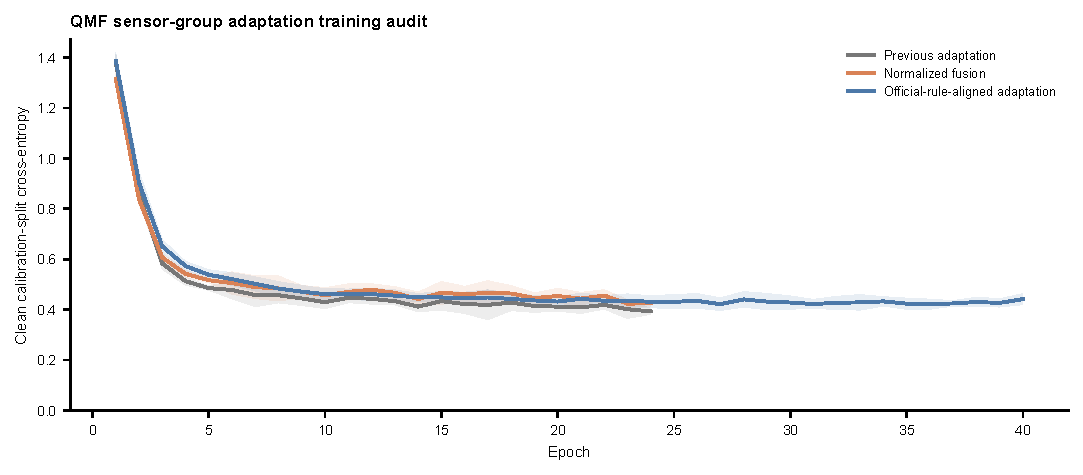
\includegraphics[width=0.92\textwidth]{figureS9_qmf_training.pdf}
\caption{\textbf{QMF sensor-group training audit.} Mean clean calibration-split cross-entropy by epoch for the previous adaptation, normalized fusion and official-rule-aligned adaptation. Ribbons are standard deviations across available repeated fits; epochs with fewer than three active fits after early stopping are omitted. The calibration split, not the held-out test set, controls checkpoint selection.}
\label{fig:supp-qmf-training}
\end{figure}

\begin{figure}[ht]
\centering
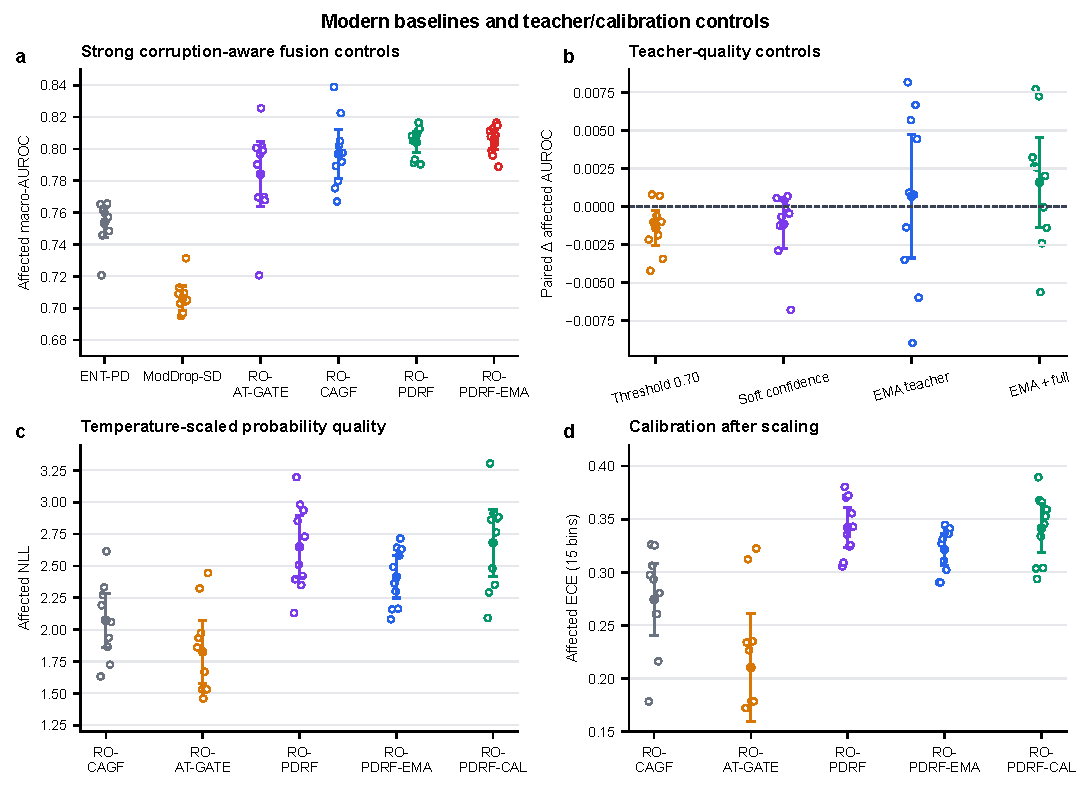
\includegraphics[width=\textwidth]{figureS7_strong_teacher_controls.pdf}
\caption{\textbf{Modern fusion and teacher/calibration controls.} \textbf{a}, Affected macro-AUROC for entropy weighting, modality-dropout self-distillation, parameter-matched attention gating, unrestricted recovery gating, bounded recovery fusion and its EMA extension. \textbf{b}, Paired affected-AUROC differences for hard-threshold, continuous-confidence and EMA teachers. \textbf{c,d}, Temperature-scaled affected NLL and ECE. Open circles are individual optimization seeds; filled circles are means and whiskers are 95\% $t$ intervals across the 10 repeated fits. The intervals describe optimization variation on one fixed test fault, not device replication.}
\label{fig:supp-strong-teacher}
\end{figure}
\FloatBarrier

\begin{table}[ht]
\centering
\caption{Original matched computational-cost audit on a 13th Gen Intel Core i5-13500H using PyTorch in CPU mode. Means and standard deviations are across three fixed seeds. Training time includes checkpoint selection; inference excludes data loading.}
\label{tab:supp-cost}
\resizebox{\textwidth}{!}{\begin{tabular}{lrrrr}
\toprule
Method & Parameters & Training time (s) & Epochs & Inference (ms/observation) \\
\midrule
CAGF & 26,588 & 10.2 $\pm$ 1.1 & 21.0 & 0.0013 $\pm$ 0.0001 \\
ENT-PD & 17,560 & 9.0 $\pm$ 2.4 & 19.0 & 0.0013 $\pm$ 0.0003 \\
PDRF & 19,740 & 13.2 $\pm$ 3.9 & 22.3 & 0.0012 $\pm$ 0.0002 \\
RO-PDRF-Full & 19,740 & 16.6 $\pm$ 4.7 & 22.3 & 0.0016 $\pm$ 0.0001 \\
\bottomrule
\end{tabular}}
\end{table}

\begin{table}[H]
\centering
\caption{Expanded measured cost audit for the principal QMF, attention, Lite, Full, EMA and teacher-safeguard runs. Times are descriptive wall-clock measurements from the same CPU software environment; early stopping creates different epoch ranges. Inference excludes data loading.}
\label{tab:supp-expanded-cost}
\resizebox{\textwidth}{!}{\begin{tabular}{lrrrr}
\toprule
Method & Parameters & Training time, mean $\pm$ SD (s) & Epochs represented & Inference (ms/observation) \\
\midrule
QMF-PD & 17,560 & 16.0 $\pm$ 3.5 & 24--47 & 0.0010 \\
RO-AT-GATE & 26,809 & 10.9 $\pm$ 3.6 & 13--30 & 0.0018 \\
RO-CAGF & 26,588 & 14.1 $\pm$ 3.0 & 15--26 & 0.0020 \\
RO-PDRF-Lite & 19,740 & 9.2 $\pm$ 2.7 & 18--41 & 0.0008 \\
RO-PDRF-Full & 19,740 & 22.7 $\pm$ 5.6 & 18--37 & 0.0020 \\
RO-PDRF-EMA & 19,740 & 23.8 $\pm$ 4.7 & 23--41 & 0.0017 \\
RO-PDRF-Full-CRA & 19,740 & 17.6 $\pm$ 5.2 & 18--41 & 0.0014 \\
RO-PDRF-Full-ECA & 19,740 & 19.3 $\pm$ 5.2 & 19--41 & 0.0014 \\
CE-conflict training audit & 19,740 & 22.0 $\pm$ 6.1 & 18--41 & 0.0018 \\
\bottomrule
\end{tabular}}
\end{table}

Lite and Full have the same 19,740 trainable parameters because their difference is objective-only. Lite required 9.2~s mean training time versus 22.7~s for Full, while one-pass inference remained below 0.002~ms per observation. QMF-PD, RO-AT-GATE and RO-PDRF-EMA required 16.0, 10.9 and 23.8~s, respectively. These measurements support Lite as the simpler practical default but are not hardware-independent complexity bounds.

\section{Fault-type, realization and EMA-decay analysis}

The expanded chemical audit crosses Gaussian noise, a featurewise signed offset, acquisition-ordered monotone drift and stuck-at replacement with eight fixed intervention realizations and five fitted seeds. Scale, affected prevalence and random group missingness remain 3, 0.40 and 0.20. Within a realization, affected rows and missingness masks are shared across fault types; all intervention values are fixed across methods. The bootstrap resamples fault type, realization within type and the crossed optimization-seed cluster, preserving that one fitted seed is evaluated under every controlled intervention. These factors describe one chemical instrument, not independent hardware.

\begin{table}[H]
\centering
\caption{Affected-subset discrimination and probability quality across four controlled fault mechanisms, eight realizations and five fitted seeds. Intervals for the EMA99 AUROC contrast use 5,000 crossed-factor bootstrap replicates.}
\label{tab:supp-fault-type-ema}
\resizebox{\textwidth}{!}{\begin{tabular}{lrrrrrr}
\toprule
Fault type & RO-CAGF AUROC & RO-PDRF-Full AUROC & EMA99 AUROC & EMA99 NLL & EMA99 ECE & $\Delta$ AUROC vs Full \\
\midrule
Drift & 0.791 & 0.826 & 0.829 & 2.139 & 0.285 & +0.003 [-0.003, +0.010] \\
Gaussian & 0.792 & 0.803 & 0.808 & 2.231 & 0.299 & +0.005 [+0.002, +0.008] \\
Offset & 0.786 & 0.816 & 0.819 & 2.382 & 0.319 & +0.003 [-0.003, +0.011] \\
Stuck-at & 0.778 & 0.811 & 0.816 & 2.247 & 0.298 & +0.004 [-0.002, +0.012] \\
\bottomrule
\end{tabular}}
\end{table}

\begin{table}[H]
\centering
\caption{Per-fault architecture effects. Intervals resample fault realization and the crossed optimization-seed cluster within each controlled mechanism. The four-type aggregate resamples only four top-level clusters and is therefore descriptive.}
\label{tab:supp-fault-architecture}
\resizebox{0.92\textwidth}{!}{\begin{tabular}{lrrr}
\toprule
Controlled fault type & RO-CAGF AUROC & RO-PDRF-Full AUROC & Difference (95\% hierarchical interval) \\
\midrule
Gaussian & 0.792 & 0.803 & +0.011 [-0.009, +0.028] \\
Offset & 0.786 & 0.816 & +0.030 [+0.003, +0.057] \\
Drift & 0.791 & 0.826 & +0.035 [+0.012, +0.057] \\
Stuck-at & 0.778 & 0.811 & +0.034 [+0.003, +0.062] \\
\midrule
Four-type descriptive aggregate & -- & -- & +0.027 [+0.002, +0.051] \\
\bottomrule
\end{tabular}}
\end{table}

\begin{table}[H]
\centering
\caption{Leave-one-fault-type-out sensitivity for the RO-PDRF-Full--RO-CAGF affected-AUROC difference. Each row has only three remaining top-level fault clusters; intervals are descriptive robustness summaries, not device-generalization intervals.}
\label{tab:supp-lofo}
\resizebox{0.84\textwidth}{!}{\begin{tabular}{lrr}
\toprule
Omitted controlled fault type & Remaining top-level clusters & RO-PDRF-Full--RO-CAGF AUROC (95\% interval) \\
\midrule
Gaussian & 3 & +0.033 [+0.007, +0.056] \\
Offset & 3 & +0.027 [+0.001, +0.052] \\
Drift & 3 & +0.025 [-0.002, +0.052] \\
Stuck-at & 3 & +0.025 [+0.000, +0.050] \\
\bottomrule
\end{tabular}}
\end{table}

Across all four mechanisms, RO-PDRF-Full exceeded RO-CAGF by a descriptive mean AUROC difference of $+0.0274$ (95\% crossed-factor interval $+0.0019$ to $+0.0512$). The per-fault effects were $+0.0112$, $+0.0299$, $+0.0351$ and $+0.0336$ for Gaussian, offset, drift and stuck-at interventions. Every leave-one-type-out mean remained positive, although the interval after omitting drift crossed zero. Only four fault mechanisms define the top level, so these results support controlled-fault breadth without estimating a population of natural failure types. Across the same design, RO-PDRF-EMA changed Full-model AUROC by $+0.0038$ ($-0.0007$ to $+0.0091$), NLL by $-0.283$ ($-0.535$ to $-0.094$) and ECE by $-0.0228$ ($-0.0396$ to $-0.0085$).

\begin{table}[H]
\centering
\caption{EMA-decay sensitivity under the principal Gaussian realization. Values are means $\pm$ standard deviations across five fitted seeds.}
\label{tab:supp-ema-decay}
\resizebox{0.72\textwidth}{!}{\begin{tabular}{lrrr}
\toprule
EMA decay & Affected AUROC & NLL & ECE \\
\midrule
0.95 & 0.807 $\pm$ 0.010 & 2.550 $\pm$ 0.214 & 0.326 $\pm$ 0.022 \\
0.99 & 0.806 $\pm$ 0.008 & 2.264 $\pm$ 0.178 & 0.301 $\pm$ 0.020 \\
0.995 & 0.805 $\pm$ 0.010 & 2.205 $\pm$ 0.077 & 0.302 $\pm$ 0.018 \\
\bottomrule
\end{tabular}}
\end{table}

\begin{figure}[p]
\centering
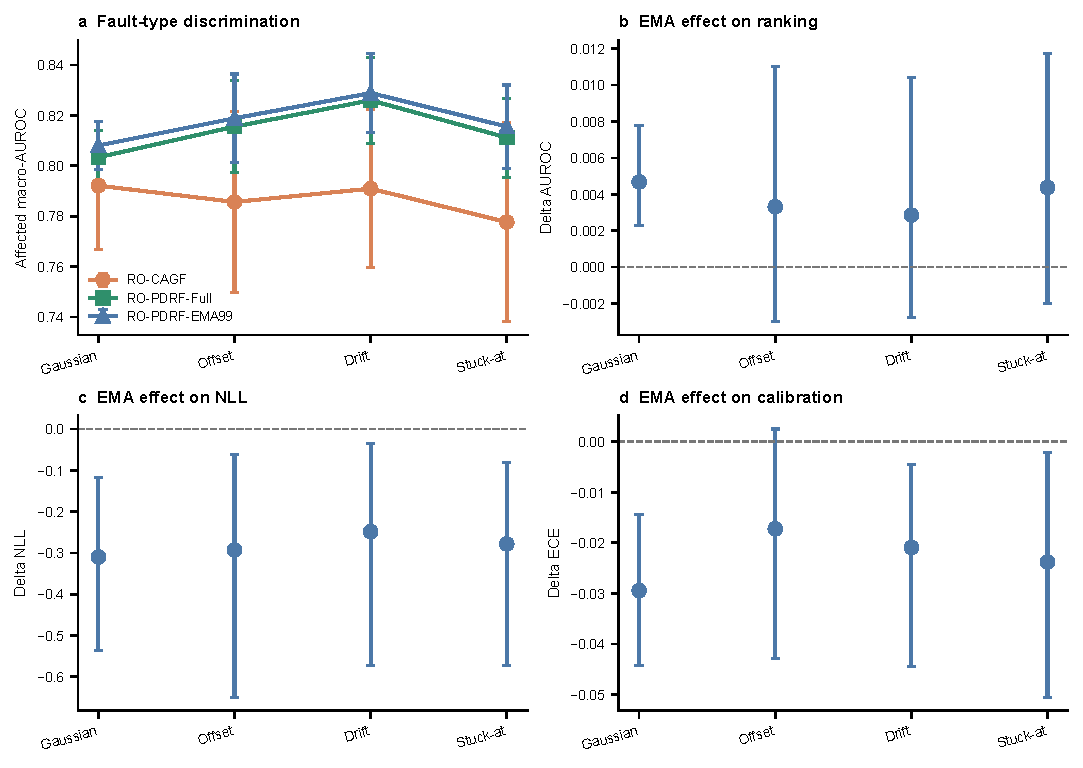
\includegraphics[width=\textwidth]{figureS8_fault_type_ema.pdf}
\caption{\textbf{Fault-type and EMA audit.} \textbf{a}, affected macro-AUROC by controlled mechanism. \textbf{b--d}, RO-PDRF-EMA minus RO-PDRF-Full effects for AUROC, NLL and ECE. Error bars use realization and crossed-seed resampling within each fault type. All interventions are repeated on one chemical instrument.}
\label{fig:supp-fault-type-ema}
\end{figure}
\FloatBarrier

\section{Score-geometry sensitivity}

The following three-seed audit changes one parameter at a time around RO-PDRF-Full. It is exploratory and was not used to replace the formal setting. A larger bound lowers outer-5\% occupancy and improves affected AUROC over this grid; larger $\beta$ improves discrimination but does not monotonically reduce saturation. Ranking weight also changes saturation materially. No single hyperparameter is therefore justified by AUROC alone.

\begin{table}[ht]
\centering
\caption{Joint score-saturation, discrimination and calibration sensitivity. Values are means across three fixed development seeds.}
\resizebox{0.92\textwidth}{!}{\begin{tabular}{lrrrrr}
\toprule
Setting & Saturation & All AUROC & Affected AUROC & NLL & ECE \\
\midrule
B=2 & 0.605 & 0.837 & 0.795 & 2.103 & 0.271 \\
B=3 & 0.556 & 0.839 & 0.801 & 2.052 & 0.268 \\
B=4 & 0.524 & 0.841 & 0.808 & 1.989 & 0.263 \\
B=5 & 0.420 & 0.845 & 0.814 & 2.019 & 0.262 \\
beta=0.1 & 0.436 & 0.831 & 0.783 & 2.150 & 0.274 \\
beta=0.25 & 0.556 & 0.839 & 0.801 & 2.052 & 0.268 \\
beta=0.5 & 0.516 & 0.850 & 0.824 & 1.932 & 0.249 \\
beta=0.75 & 0.612 & 0.853 & 0.832 & 1.905 & 0.253 \\
rank=0.05 & 0.294 & 0.832 & 0.790 & 2.150 & 0.272 \\
rank=0.15 & 0.556 & 0.839 & 0.801 & 2.052 & 0.268 \\
rank=0.3 & 0.650 & 0.840 & 0.804 & 2.113 & 0.274 \\
\bottomrule
\end{tabular}}
\end{table}

\section{Hydraulic no-interpolation audit}

The principal hydraulic representation linearly resamples each physical-group summary vector to length 48. The no-interpolation audit instead retains every native summary value in its original order and zero-pads only the unused tail. Both representations use identical samples, splits, faults and seeds.

\begin{table}[ht]
\centering
\caption{Affected-subset macro-AUROC under controlled hydraulic pressure faults. Difference is RO-PDRF-NOQ minus CAGF.}
\resizebox{0.82\textwidth}{!}{\begin{tabular}{llrrr}
\toprule
Representation & Task & CAGF & RO-PDRF-Full & Difference \\
\midrule
Linear resampling & Accumulator & 0.608 & 0.693 & +0.085 \\
Linear resampling & Cooler & 0.949 & 1.000 & +0.051 \\
Linear resampling & Pump & 0.871 & 0.921 & +0.050 \\
Linear resampling & Valve & 0.697 & 0.684 & -0.013 \\
No interpolation & Accumulator & 0.575 & 0.710 & +0.135 \\
No interpolation & Cooler & 0.919 & 1.000 & +0.081 \\
No interpolation & Pump & 0.787 & 0.911 & +0.124 \\
No interpolation & Valve & 0.681 & 0.656 & -0.025 \\
\bottomrule
\end{tabular}}
\end{table}

\section{Real-operational AHU direct-diagnosis boundary analysis}

The external field audit uses one year of hourly operational records from each of three buildings and only the repository's expert annotations for normal operation, return-air temperature sensor fault and supply-air temperature sensor fault. No test fault is synthesized. Table~\ref{tab:supp-ahu-splits} reports the chronological partitions after exclusion of conflicting duplicate AHU--time keys and collapse of same-label repeats. The complete test periods are retained without class subsampling.

For leave-one-building-out analysis, models train on two buildings and hold out the third. Shift diagnostics include standardized mean, variance, quantile, missingness and outlier differences per feature; Kolmogorov--Smirnov and Wasserstein distances; linear and radial-basis maximum mean discrepancy; covariance discrepancy; a source-trained PCA projection; and class/subtype priors. A reversal audit reports AUROC from $1-p(\mathrm{fault})$ to distinguish absent ranking information from approximately inverted ranking. Source-only controls use source normalization and include EF-PD, RO-PDRF-Full-NOQ and GroupDRO-EF-PD with building as the source group. Target normalization recomputes location and scale from unlabeled target features, while CORAL aligns source covariance to unlabeled target covariance. These two regimes are unsupervised target adaptation, not source-only transfer.

Five-member probabilities are averaged for risk--coverage analysis. Split-conformal sets use calibration nonconformity $1-p_y$ at nominal error levels 0.05, 0.10 and 0.20. Empirical coverage, mean set size, singleton rate and singleton accuracy are diagnostics only because chronological and cross-building shift violate simple exchangeability.

\begin{table}[ht]
\centering
\caption{Chronological AHU split counts used in the field validation.}
\label{tab:supp-ahu-splits}
\resizebox{0.72\textwidth}{!}{\begin{tabular}{llrrr}
\toprule
Building & Split & Records & Normal & Sensor fault \\
\midrule
Auditorium & Train & 7,658 & 6,000 & 1,658 \\
Auditorium & Selection & 1,728 & 1,500 & 228 \\
Auditorium & Calibration & 1,524 & 1,500 & 24 \\
Auditorium & Test & 9,354 & 9,126 & 228 \\
Hospital & Train & 11,300 & 6,000 & 5,300 \\
Hospital & Selection & 2,675 & 1,500 & 1,175 \\
Hospital & Calibration & 2,318 & 1,500 & 818 \\
Hospital & Test & 9,362 & 7,867 & 1,495 \\
Office & Train & 11,727 & 6,000 & 5,727 \\
Office & Selection & 3,000 & 1,500 & 1,500 \\
Office & Calibration & 1,755 & 1,500 & 255 \\
Office & Test & 19,115 & 18,769 & 346 \\
\bottomrule
\end{tabular}
}
\end{table}

\begin{table}[ht]
\centering
\caption{Class and native sensor-fault-subtype distribution in each untouched chronological test period.}
\label{tab:supp-ahu-distribution}
\resizebox{0.72\textwidth}{!}{\begin{tabular}{lrrrr}
\toprule
Building & Normal & Return-air fault & Supply-air fault & Total \\
\midrule
Auditorium & 9,126 & 179 & 49 & 9,354 \\
Hospital & 7,867 & 1,487 & 8 & 9,362 \\
Office & 18,769 & 293 & 53 & 19,115 \\
\bottomrule
\end{tabular}}
\end{table}

The hospital test period is qualitatively different from the other two buildings: it contains 1,487 return-air faults but only eight supply-air faults. Metrics are therefore reported by building and subtype rather than pooled across hourly observations.

\begin{table}[ht]
\centering
\caption{Detailed chronological AHU results. Values are means across five matched seeds. Fault precision, recall and F1 treat either native temperature-sensor-fault subtype as the positive class.}
\label{tab:supp-ahu-detailed}
\resizebox{\textwidth}{!}{\begin{tabular}{llrrrrrrr}
\toprule
Building & Method & AUROC & AUPRC & Macro-F1 & Bal. Acc. & Fault Prec. & Fault Recall & Fault F1 \\
\midrule
Auditorium & EF-PD & 0.996 & 0.957 & 0.901 & 0.913 & 0.793 & 0.832 & 0.807 \\
Auditorium & HGB-current & 0.993 & 0.932 & 0.854 & 0.941 & 0.598 & 0.896 & 0.717 \\
Auditorium & HGB-lag & 0.992 & 0.925 & 0.863 & 0.871 & 0.720 & 0.749 & 0.733 \\
Auditorium & ENT-PD & 0.980 & 0.833 & 0.755 & 0.893 & 0.395 & 0.818 & 0.529 \\
Auditorium & CAGF & 0.990 & 0.907 & 0.832 & 0.861 & 0.666 & 0.733 & 0.674 \\
Auditorium & PDRF-NOQ & 0.985 & 0.812 & 0.695 & 0.954 & 0.271 & 0.973 & 0.424 \\
Auditorium & RO-PDRF-Full-NOQ & 0.984 & 0.809 & 0.698 & 0.943 & 0.276 & 0.947 & 0.428 \\
\addlinespace
Hospital & EF-PD & 0.990 & 0.983 & 0.947 & 0.926 & 0.969 & 0.857 & 0.909 \\
Hospital & HGB-current & 0.978 & 0.968 & 0.946 & 0.921 & 0.983 & 0.845 & 0.909 \\
Hospital & HGB-lag & 0.964 & 0.958 & 0.941 & 0.911 & 0.993 & 0.822 & 0.899 \\
Hospital & ENT-PD & 0.958 & 0.950 & 0.935 & 0.909 & 0.965 & 0.824 & 0.889 \\
Hospital & CAGF & 0.912 & 0.928 & 0.943 & 0.913 & 0.995 & 0.828 & 0.903 \\
Hospital & PDRF-NOQ & 0.936 & 0.939 & 0.941 & 0.909 & 1.000 & 0.817 & 0.899 \\
Hospital & RO-PDRF-Full-NOQ & 0.931 & 0.937 & 0.940 & 0.908 & 1.000 & 0.815 & 0.898 \\
\addlinespace
Office & EF-PD & 0.998 & 0.945 & 0.816 & 0.987 & 0.481 & 0.995 & 0.642 \\
Office & HGB-current & 0.996 & 0.897 & 0.756 & 0.984 & 0.360 & 1.000 & 0.529 \\
Office & HGB-lag & 0.996 & 0.882 & 0.756 & 0.984 & 0.359 & 1.000 & 0.528 \\
Office & ENT-PD & 0.975 & 0.727 & 0.786 & 0.869 & 0.479 & 0.753 & 0.581 \\
Office & CAGF & 0.984 & 0.845 & 0.770 & 0.967 & 0.422 & 0.971 & 0.559 \\
Office & PDRF-NOQ & 0.968 & 0.709 & 0.630 & 0.950 & 0.180 & 0.983 & 0.304 \\
Office & RO-PDRF-Full-NOQ & 0.966 & 0.704 & 0.620 & 0.914 & 0.169 & 0.912 & 0.285 \\
\addlinespace
\bottomrule
\end{tabular}}
\end{table}

\begin{table}[ht]
\centering
\caption{Recall for the two native expert-annotated fault subtypes. The class counts in Table~\ref{tab:supp-ahu-distribution} govern interpretation, especially for the eight hospital supply-air faults.}
\label{tab:supp-ahu-subtypes}
\resizebox{0.86\textwidth}{!}{\begin{tabular}{lllrr}
\toprule
Building & Method & Fault subtype & Recall & Number of seeds \\
\midrule
Auditorium & EF-PD & Return-air & 0.785 $\pm$ 0.097 & 5 \\
Auditorium & EF-PD & Supply-air & 1.000 $\pm$ 0.000 & 5 \\
Auditorium & HGB-current & Return-air & 0.873 $\pm$ 0.024 & 5 \\
Auditorium & HGB-current & Supply-air & 0.984 $\pm$ 0.009 & 5 \\
Auditorium & HGB-lag & Return-air & 0.685 $\pm$ 0.045 & 5 \\
Auditorium & HGB-lag & Supply-air & 0.984 $\pm$ 0.027 & 5 \\
Auditorium & ENT-PD & Return-air & 0.783 $\pm$ 0.108 & 5 \\
Auditorium & ENT-PD & Supply-air & 0.947 $\pm$ 0.031 & 5 \\
Auditorium & CAGF & Return-air & 0.667 $\pm$ 0.171 & 5 \\
Auditorium & CAGF & Supply-air & 0.976 $\pm$ 0.037 & 5 \\
Auditorium & PDRF-NOQ & Return-air & 0.965 $\pm$ 0.009 & 5 \\
Auditorium & PDRF-NOQ & Supply-air & 1.000 $\pm$ 0.000 & 5 \\
Auditorium & RO-PDRF-Full-NOQ & Return-air & 0.933 $\pm$ 0.012 & 5 \\
Auditorium & RO-PDRF-Full-NOQ & Supply-air & 1.000 $\pm$ 0.000 & 5 \\
Hospital & EF-PD & Return-air & 0.862 $\pm$ 0.020 & 5 \\
Hospital & EF-PD & Supply-air & 0.000 $\pm$ 0.000 & 5 \\
Hospital & HGB-current & Return-air & 0.846 $\pm$ 0.003 & 5 \\
Hospital & HGB-current & Supply-air & 0.675 $\pm$ 0.381 & 5 \\
Hospital & HGB-lag & Return-air & 0.827 $\pm$ 0.001 & 5 \\
Hospital & HGB-lag & Supply-air & 0.000 $\pm$ 0.000 & 5 \\
Hospital & ENT-PD & Return-air & 0.828 $\pm$ 0.002 & 5 \\
Hospital & ENT-PD & Supply-air & 0.000 $\pm$ 0.000 & 5 \\
Hospital & CAGF & Return-air & 0.832 $\pm$ 0.024 & 5 \\
Hospital & CAGF & Supply-air & 0.000 $\pm$ 0.000 & 5 \\
Hospital & PDRF-NOQ & Return-air & 0.822 $\pm$ 0.002 & 5 \\
Hospital & PDRF-NOQ & Supply-air & 0.000 $\pm$ 0.000 & 5 \\
Hospital & RO-PDRF-Full-NOQ & Return-air & 0.820 $\pm$ 0.005 & 5 \\
Hospital & RO-PDRF-Full-NOQ & Supply-air & 0.000 $\pm$ 0.000 & 5 \\
Office & EF-PD & Return-air & 0.994 $\pm$ 0.008 & 5 \\
Office & EF-PD & Supply-air & 1.000 $\pm$ 0.000 & 5 \\
Office & HGB-current & Return-air & 1.000 $\pm$ 0.000 & 5 \\
Office & HGB-current & Supply-air & 1.000 $\pm$ 0.000 & 5 \\
Office & HGB-lag & Return-air & 1.000 $\pm$ 0.000 & 5 \\
Office & HGB-lag & Supply-air & 1.000 $\pm$ 0.000 & 5 \\
Office & ENT-PD & Return-air & 0.792 $\pm$ 0.071 & 5 \\
Office & ENT-PD & Supply-air & 0.532 $\pm$ 0.117 & 5 \\
Office & CAGF & Return-air & 0.966 $\pm$ 0.050 & 5 \\
Office & CAGF & Supply-air & 1.000 $\pm$ 0.000 & 5 \\
Office & PDRF-NOQ & Return-air & 0.992 $\pm$ 0.002 & 5 \\
Office & PDRF-NOQ & Supply-air & 0.932 $\pm$ 0.077 & 5 \\
Office & RO-PDRF-Full-NOQ & Return-air & 0.965 $\pm$ 0.020 & 5 \\
Office & RO-PDRF-Full-NOQ & Supply-air & 0.619 $\pm$ 0.130 & 5 \\
\bottomrule
\end{tabular}}
\end{table}

\begin{table}[ht]
\centering
\caption{Confusion counts for fixed five-member probability ensembles on the untouched chronological test periods. Either native sensor-fault subtype is positive.}
\label{tab:supp-ahu-confusion}
\resizebox{0.76\textwidth}{!}{\begin{tabular}{llrrrr}
\toprule
Building & Method & TN & FP & FN & TP \\
\midrule
Auditorium & EF-PD & 9,080 & 46 & 41 & 187 \\
Auditorium & HGB-current & 9,000 & 126 & 23 & 205 \\
Auditorium & HGB-lag & 9,061 & 65 & 55 & 173 \\
Auditorium & ENT-PD & 8,824 & 302 & 36 & 192 \\
Auditorium & CAGF & 9,072 & 54 & 70 & 158 \\
Auditorium & RO-PDRF-Full-NOQ & 8,557 & 569 & 11 & 217 \\
\addlinespace
Hospital & EF-PD & 7,853 & 14 & 214 & 1,281 \\
Hospital & HGB-current & 7,848 & 19 & 232 & 1,263 \\
Hospital & HGB-lag & 7,860 & 7 & 267 & 1,228 \\
Hospital & ENT-PD & 7,866 & 1 & 262 & 1,233 \\
Hospital & CAGF & 7,866 & 1 & 273 & 1,222 \\
Hospital & RO-PDRF-Full-NOQ & 7,867 & 0 & 274 & 1,221 \\
\addlinespace
Office & EF-PD & 18,426 & 343 & 1 & 345 \\
Office & HGB-current & 18,166 & 603 & 0 & 346 \\
Office & HGB-lag & 18,157 & 612 & 0 & 346 \\
Office & ENT-PD & 18,458 & 311 & 78 & 268 \\
Office & CAGF & 18,378 & 391 & 2 & 344 \\
Office & RO-PDRF-Full-NOQ & 17,259 & 1,510 & 29 & 317 \\
\addlinespace
\bottomrule
\end{tabular}}
\end{table}

Table~\ref{tab:supp-ahu-tests} treats the 15 building--seed combinations as matched repeated fits. These tests describe optimization consistency across the three building-specific tasks; they do not treat hourly records as independent retraining replicates. EF-PD and HGB-current exceed RO-PDRF-NOQ in all 15 pairs. HGB-lag does not uniformly improve HGB-current, showing that these fixed lag summaries are a task-specific baseline rather than a surrogate for every sequence architecture.

\begin{table}[ht]
\centering
\caption{Paired AHU macro-AUROC contrasts for RO-PDRF-NOQ across five seeds and three buildings.}
\label{tab:supp-ahu-tests}
\resizebox{0.72\textwidth}{!}{\begin{tabular}{lrrrr}
\toprule
Contrast & Mean $\Delta$ AUROC & Wins & Losses & Exact $P$ \\
\midrule
RO-PDRF-Full-NOQ vs. PDRF-NOQ & -0.0023 & 2 & 13 & 0.0006 \\
RO-PDRF-Full-NOQ vs. CAGF & -0.0018 & 6 & 9 & 0.8040 \\
RO-PDRF-Full-NOQ vs. ENT-PD & -0.0104 & 5 & 10 & 0.0479 \\
RO-PDRF-Full-NOQ vs. EF-PD & -0.0341 & 0 & 15 & 0.0001 \\
RO-PDRF-Full-NOQ vs. UF-PD & -0.0066 & 7 & 8 & 0.1514 \\
RO-PDRF-Full-NOQ vs. HGB-current & -0.0285 & 0 & 15 & 0.0001 \\
RO-PDRF-Full-NOQ vs. HGB-lag & -0.0235 & 0 & 15 & 0.0001 \\
\bottomrule
\end{tabular}
}
\end{table}

\begin{table}[ht]
\centering
\caption{Split-conformal diagnostics at nominal error level $\alpha=0.10$. Calibration uses the chronological calibration interval and evaluation uses the later test interval.}
\label{tab:supp-ahu-conformal}
\resizebox{\textwidth}{!}{\begin{tabular}{llrrrr}
\toprule
Building & Method & Coverage & Mean set size & Singleton rate & Singleton accuracy \\
\midrule
Auditorium & CAGF & 0.674 & 0.674 & 0.674 & 1.000 \\
Auditorium & EF-PD & 0.832 & 0.832 & 0.832 & 1.000 \\
Auditorium & ENT-PD & 0.548 & 0.548 & 0.548 & 1.000 \\
Auditorium & HGB-lag & 0.627 & 0.627 & 0.627 & 1.000 \\
Auditorium & RO-PDRF-Full-NOQ & 0.525 & 0.525 & 0.525 & 1.000 \\
Hospital & CAGF & 0.586 & 0.597 & 0.597 & 0.981 \\
Hospital & EF-PD & 0.983 & 1.017 & 0.983 & 0.983 \\
Hospital & ENT-PD & 0.520 & 0.523 & 0.523 & 0.995 \\
Hospital & HGB-lag & 0.637 & 0.639 & 0.639 & 0.996 \\
Hospital & RO-PDRF-Full-NOQ & 0.875 & 0.902 & 0.902 & 0.970 \\
Office & CAGF & 0.868 & 0.868 & 0.868 & 1.000 \\
Office & EF-PD & 0.829 & 0.830 & 0.830 & 0.999 \\
Office & ENT-PD & 0.916 & 0.921 & 0.921 & 0.994 \\
Office & HGB-lag & 0.939 & 0.944 & 0.944 & 0.995 \\
Office & RO-PDRF-Full-NOQ & 0.918 & 0.998 & 0.998 & 0.920 \\
\bottomrule
\end{tabular}}
\end{table}

Empirical coverage is frequently below the nominal 0.90 target, most notably in the auditorium. This is evidence against claiming a distribution-free field guarantee: chronological changes violate the exchangeability condition needed for the elementary split-conformal construction. Confidence-based abstention can still reduce selective error, but confidence ordering and class-specific recall must be audited together.

\begin{figure}[ht]
\centering
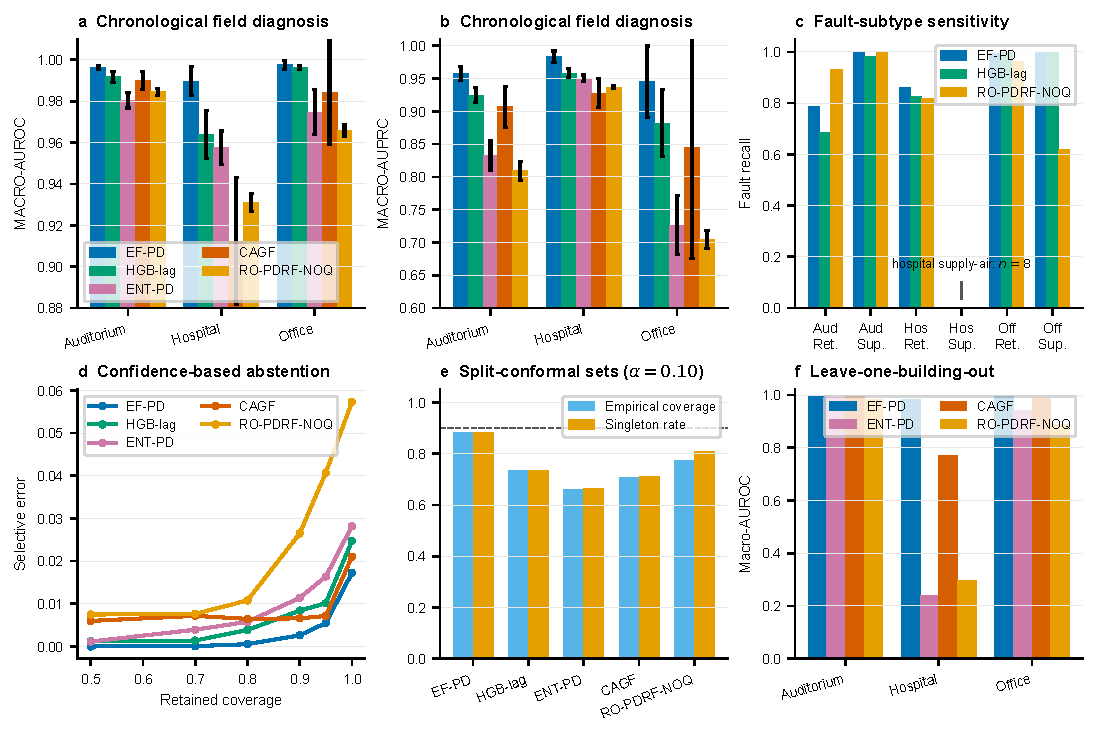
\includegraphics[width=\textwidth]{figureS1_ahu_field_diagnostics.pdf}
\caption{\textbf{Operational AHU diagnosis and deployment boundaries.} \textbf{a,b}, Building-specific chronological AUROC and AUPRC. \textbf{c}, Return- and supply-air fault recall, with the rare hospital supply-air subset identified. \textbf{d}, Selective error as lower-confidence predictions are rejected. \textbf{e}, Empirical split-conformal coverage and singleton rate at nominal 90\% coverage. \textbf{f}, leave-one-building-out AUROC without target-building adaptation. Error bars in \textbf{a--c} show standard deviations across five seeds.}
\label{fig:supp-ahu}
\end{figure}

A deliberately harder leave-one-building-out audit trains on two buildings and evaluates the third without target-building adaptation. The five-seed results in Table~\ref{tab:supp-ahu-domain} show substantial domain shift, especially for the hospital. This audit is not used to select the temporal protocol or to claim device-independent transfer; it identifies a deployment boundary that requires explicit domain adaptation.

\begin{table}[ht]
\centering
\caption{Leave-one-building-out macro-AUROC averaged across five fixed seeds.}
\label{tab:supp-ahu-domain}
\resizebox{0.78\textwidth}{!}{\begin{tabular}{lccccc}
\toprule
Held-out building & EF-PD & ENT-PD & CAGF & PDRF-NOQ & RO-PDRF-Full-NOQ \\
\midrule
Auditorium & 1.000 $\pm$ 0.000 & 0.990 $\pm$ 0.001 & 1.000 $\pm$ 0.000 & 0.983 $\pm$ 0.001 & 0.984 $\pm$ 0.000 \\
Hospital & 0.983 $\pm$ 0.003 & 0.238 $\pm$ 0.012 & 0.772 $\pm$ 0.167 & 0.302 $\pm$ 0.004 & 0.298 $\pm$ 0.005 \\
Office & 0.994 $\pm$ 0.002 & 0.941 $\pm$ 0.007 & 0.986 $\pm$ 0.002 & 0.884 $\pm$ 0.006 & 0.887 $\pm$ 0.006 \\
\bottomrule
\end{tabular}
}
\end{table}

The failure is concentrated rather than hidden by an overall average. RO-PDRF-NOQ retained AUROC $0.984\pm0.000$ for the held-out auditorium and $0.887\pm0.006$ for the held-out office, but fell to $0.298\pm0.005$ for the hospital. ENT-PD and PDRF-NOQ failed similarly on the hospital, whereas EF-PD retained $0.983\pm0.003$. The learned bounded-score pathway therefore did not align across the hospital domain.

The expanded audit diagnoses this boundary instead of assuming that one adaptation is sufficient. Reversed hospital RO-PDRF-Full-NOQ probabilities yield AUROC $0.702\pm0.005$, revealing approximately inverted ranking. Target normalization and CORAL improve the original AUROC only to $0.356\pm0.005$ and $0.367\pm0.006$ and therefore do not repair it. GroupDRO-EF-PD remains strong at $0.982\pm0.004$ but does not improve on source-normalized EF-PD. Full feature-level shifts, PCA coordinates, prediction files and risk--coverage traces are supplied as source data.

\begin{table}[ht]
\centering
\caption{Multivariate leave-one-building-out shift distances. Values are descriptive distances computed without target labels.}
\resizebox{0.76\textwidth}{!}{\begin{tabular}{lrrr}
\toprule
Held-out building & Linear MMD & RBF MMD & CORAL distance \\
\midrule
Auditorium & 1.448 & 0.133 & 0.00062 \\
Hospital & 3.102 & 0.198 & 0.00104 \\
Office & 1.354 & 0.073 & 0.00106 \\
\bottomrule
\end{tabular}}
\end{table}

\begin{table}[ht]
\centering
\caption{Largest hospital feature shifts under source normalization, including location, dispersion, missingness and outlier diagnostics.}
\resizebox{\textwidth}{!}{\begin{tabular}{lrrrr}
\toprule
Feature & Standardized mean difference & KS & Wasserstein & Target outside source 1--99\% \\
\midrule
cooling pump & +2.52 & 0.98 & 0.71 & 0.0\% \\
set point temperature & +1.24 & 0.61 & 2.91 & 0.0\% \\
return temperature & +1.01 & 0.45 & 2.93 & 0.4\% \\
supply fan & +0.63 & 0.34 & 0.29 & 0.0\% \\
supply air temperature & +0.60 & 0.35 & 2.95 & 1.4\% \\
heating supply temperature & +0.58 & 0.38 & 6.81 & 15.1\% \\
valve position & -0.47 & 0.17 & 10.30 & 0.0\% \\
cooling supply temperature & -0.12 & 0.44 & 4.03 & 19.1\% \\
\bottomrule
\end{tabular}}
\end{table}

\begin{figure}[p]
\centering
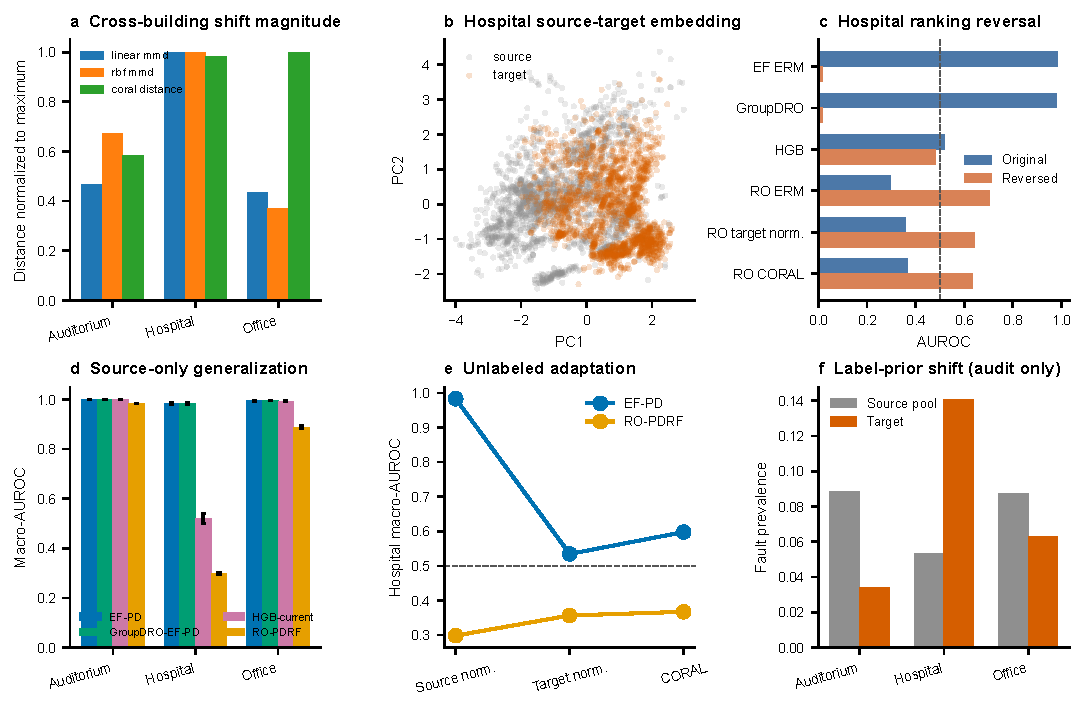
\includegraphics[width=\textwidth]{figureS2_ahu_shift_adaptation.pdf}
\caption{\textbf{Full cross-building shift and adaptation audit.} Panels report source-trained PCA geometry, multivariate distances, feature-level shifts, source/target class and subtype priors, five-seed direct-diagnosis AUROC, hospital reversed-score AUROC and selective-risk behaviour. Target normalization and CORAL use unlabeled target features and are not zero-shot methods.}
\label{fig:supp-ahu-shift}
\end{figure}
\FloatBarrier

\section{Protocol reconciliation and recovery-objective controls}

The legacy unified assignment protocol uses the clean-view teacher, fixed chemical test-fault seed 70001 and the same 10 optimization seeds for CAGF, RO-CAGF, PDRF and RO-PDRF-Full. An original recovery/calibration run used the same test fault but a label-assisted teacher for the bounded recovery model. A superseded factorial rerun used a different fixed test-fault instance (seed 85000). The latter difference changed the assigned rows and explains why nominally identical legacy source-data identifiers previously had different values. Table~\ref{tab:supp-protocol} records every relevant protocol field. The revised main paper reuses the unified fitted models but restricts evaluation to fault-applied-and-available rows.

\begin{table}[ht]
\centering
\caption{Reconciliation of the original formal run, superseded factorial rerun and legacy unified assignment protocol. CE denotes cross-entropy.}
\label{tab:supp-protocol}
\resizebox{\textwidth}{!}{\begin{tabular}{llll}
\toprule
Protocol field & Original formal run & Superseded rerun & Unified headline \\
\midrule
Purpose & recovery/calibration audit & initial 2$\times$2 audit & sole main-paper protocol \\
Recovery teacher & label-assisted best view & label-assisted best view & clean view \\
Chemical seeds & 101--110 & 101--110 & 101--110 \\
Data split indices & batches 1--6 / 7 / 8--10 & same & same \\
Initialization & PyTorch seed 101--110 & same & same \\
Test-fault seed & 70001 & 85000 & 70001 \\
Fault / group & Gaussian scale 3 / group 1 & Gaussian scale 3 / group 1 & Gaussian scale 3 / group 1 \\
Affected / missing & 40\% / 20\% & 40\% / 20\% & 40\% / 20\% \\
Quality at test & neutral ($q=1$) & neutral ($q=1$) & neutral ($q=1$) \\
Checkpoint & natural selection CE & natural selection CE & natural selection CE \\
Training / inference paths & 3 / 1 & 3 / 1 & 3 / 1 \\
Evaluation subset & fixed affected rows & different fixed affected rows & fixed affected rows \\
Status & supplementary sensitivity & archived / superseded & headline \\
\bottomrule
\end{tabular}}
\end{table}

The recovery-objective-matched $2\times2$ comparison applies clean-view recovery distillation, Brier supervision and degraded-view ranking to both bounded PDRF and unrestricted CAGF. It remains architecture-specific because RO-PDRF-Full uses a response-interior penalty while RO-CAGF uses a gate KL penalty. The seed-level contrasts and CPU cost below complement the main paper. Exact tests remain descriptive, and the 17 chemical stress conditions are correlated sensitivity conditions rather than independent replications.

\begin{table}[ht]
\centering
\caption{Recovery-objective-matched chemical and hydraulic contrasts. Positive values favour the first named method.}
\resizebox{\textwidth}{!}{\begin{tabular}{llrrrr}
\toprule
Dataset & Contrast & Mean $\Delta$ AUROC (95\% CI) & Wins & Losses & $P$ \\
\midrule
Chemical & RO-PDRF-Full - PDRF & +0.014 [+0.011, +0.016] & 10 & 0 & 0.0020 \\
Chemical & RO-CAGF - CAGF & +0.005 [-0.008, +0.017] & 6 & 4 & 0.3750 \\
Chemical & RO-PDRF-Full - RO-CAGF & +0.007 [-0.004, +0.018] & 7 & 3 & 0.3223 \\
Chemical & PDRF - CAGF & -0.001 [-0.014, +0.011] & 5 & 5 & 0.9219 \\
Chemical & interaction: bounded recovery gain - gate recovery gain & +0.008 [-0.003, +0.020] & 7 & 3 & 0.2324 \\
Hydraulic & RO-PDRF-Full - RO-CAGF & +0.044 [+0.016, +0.068] & 7 & 1 & 0.0391 \\
Hydraulic & RO-PDRF-Full - PDRF & +0.008 [-0.003, +0.021] & 3 & 3 & 0.5625 \\
Hydraulic & RO-CAGF - CAGF & +0.027 [+0.010, +0.047] & 8 & 0 & 0.0078 \\
\bottomrule
\end{tabular}}
\end{table}

\begin{table}[ht]
\centering
\caption{Recovery-objective-matched parameter counts and measured CPU costs. All four methods use three forward paths during training and one during inference.}
\resizebox{0.90\textwidth}{!}{\begin{tabular}{llrrrr}
\toprule
Dataset & Method & Parameters & Train time (s) & Inference (ms/obs.) & Training paths \\
\midrule
Chemical & CAGF & 26,588 & 13.5 $\pm$ 4.0 & 0.0019 $\pm$ 0.0003 & 3 \\
Chemical & PDRF & 19,740 & 18.1 $\pm$ 5.9 & 0.0020 $\pm$ 0.0002 & 3 \\
Chemical & RO-CAGF & 26,588 & 14.1 $\pm$ 3.0 & 0.0020 $\pm$ 0.0002 & 3 \\
Chemical & RO-PDRF-Full & 19,740 & 22.7 $\pm$ 5.6 & 0.0020 $\pm$ 0.0002 & 3 \\
Hydraulic & CAGF & 37,844 & 7.5 $\pm$ 2.4 & 0.0116 $\pm$ 0.0011 & 3 \\
Hydraulic & PDRF & 29,300 & 10.4 $\pm$ 1.8 & 0.0115 $\pm$ 0.0010 & 3 \\
Hydraulic & RO-CAGF & 37,844 & 8.5 $\pm$ 3.0 & 0.0145 $\pm$ 0.0054 & 3 \\
Hydraulic & RO-PDRF-Full & 29,300 & 11.8 $\pm$ 1.9 & 0.0119 $\pm$ 0.0019 & 3 \\
\bottomrule
\end{tabular}}
\end{table}

The clean-view teacher is the formal model. Label-assisted best-view, affected-group-removal and confidence-selected teachers are sensitivity variants evaluated on their own prespecified fixed fault (seed 87001), separate from the seed-70001 headline fault. Their near-identical affected-subset performance within that matched sensitivity experiment shows that its result does not depend materially on teacher selection; it is not pooled with the headline comparison. A separate leave-one-loss-out audit removes recovery distillation, Brier, interior or degraded-AUC supervision one at a time from the clean-teacher objective under the headline fault.

\begin{table}[ht]
\centering
\caption{Recovery-teacher audit across 10 matched chemical-array seeds. Clean-only is the formal teacher; best-CE uses training labels and is retained only as sensitivity.}
\resizebox{0.84\textwidth}{!}{\begin{tabular}{lrrr}
\toprule
Teacher selection & Aff. AUROC & Aff. AUPRC & Aff. NLL \\
\midrule
clean only & 0.823 $\pm$ 0.010 & 0.551 $\pm$ 0.018 & 2.425 $\pm$ 0.300 \\
best ce & 0.823 $\pm$ 0.010 & 0.552 $\pm$ 0.018 & 2.459 $\pm$ 0.305 \\
removal only & 0.822 $\pm$ 0.010 & 0.551 $\pm$ 0.018 & 2.457 $\pm$ 0.299 \\
confidence selected & 0.823 $\pm$ 0.010 & 0.550 $\pm$ 0.020 & 2.417 $\pm$ 0.306 \\
\bottomrule
\end{tabular}}
\end{table}

\begin{table}[ht]
\centering
\caption{Leave-one-loss-out affected-AUROC contrasts. Positive full-minus-ablated differences favour the complete recovery objective.}
\resizebox{0.82\textwidth}{!}{\begin{tabular}{lrrrr}
\toprule
Omitted term & Full-minus-ablated AUROC (95\% CI) & Wins & Losses & $P$ \\
\midrule
Recovery & +0.010 [+0.008, +0.013] & 10 & 0 & 0.0020 \\
Brier & +0.002 [+0.001, +0.003] & 9 & 1 & 0.0098 \\
Interior & +0.001 [-0.000, +0.002] & 6 & 4 & 0.2754 \\
Auc & +0.002 [+0.001, +0.004] & 8 & 2 & 0.0645 \\
\bottomrule
\end{tabular}}
\end{table}

\begin{figure}[ht]
\centering
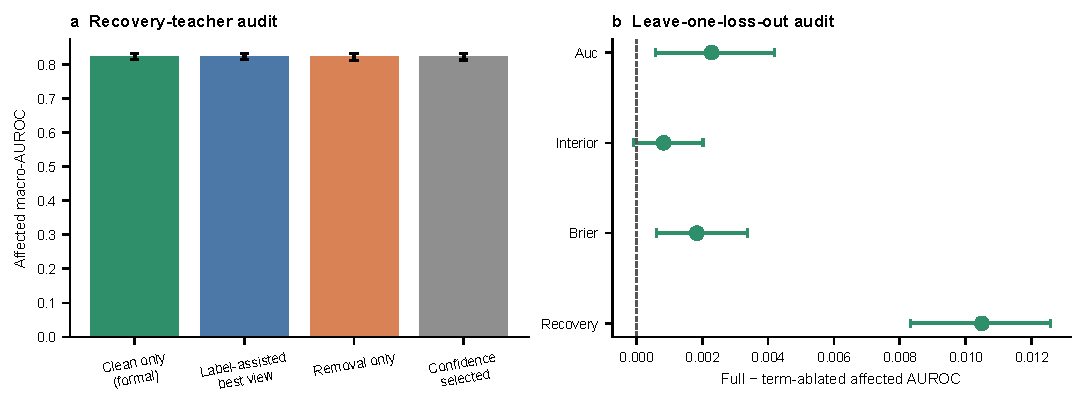
\includegraphics[width=\textwidth]{figureS3_recovery_objective_ablation.pdf}
\caption{\textbf{Recovery-objective robustness.} \textbf{a}, affected macro-AUROC under four teacher rules. \textbf{b}, paired full-objective minus leave-one-loss-out effects. Error bars show standard deviations or paired 95\% bootstrap intervals as indicated.}
\label{fig:supp-objective-ablation}
\end{figure}

The architecture-specific penalties are tested at weights 0, 0.001, 0.005 and 0.020. The complete $4\times4$ contrast matrix prevents the architecture conclusion from depending on one selected KL/interior pair.

\begin{table}[ht]
\centering
\caption{Architecture-specific regularizer sensitivity under the unique chemical headline protocol.}
\resizebox{0.78\textwidth}{!}{\begin{tabular}{lrr}
\toprule
Recovery model / regularizer weight & Aff. AUROC & SD \\
\midrule
RO-CAGF KL=0 & 0.796 & 0.031 \\
RO-CAGF KL=.001 & 0.795 & 0.028 \\
RO-CAGF KL=.005 & 0.797 & 0.022 \\
RO-CAGF KL=.020 & 0.799 & 0.018 \\
RO-PDRF-Full interior=0 & 0.803 & 0.009 \\
RO-PDRF-Full interior=.001 & 0.804 & 0.009 \\
RO-PDRF-Full interior=.005 & 0.804 & 0.009 \\
RO-PDRF-Full interior=.020 & 0.805 & 0.009 \\
\bottomrule
\end{tabular}}
\end{table}

\begin{figure}[ht]
\centering
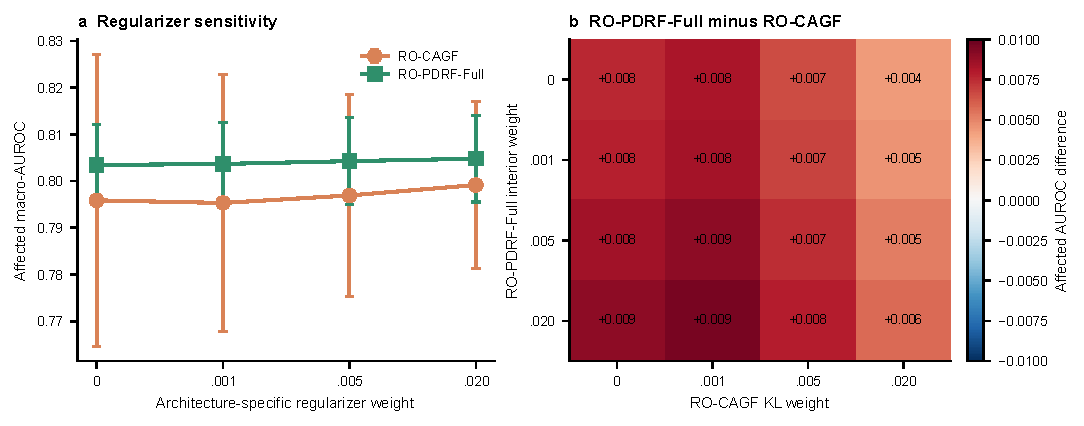
\includegraphics[width=\textwidth]{figureS4_regularizer_sensitivity.pdf}
\caption{\textbf{Architecture-specific regularizer sensitivity.} \textbf{a}, affected macro-AUROC across gate-KL and bounded-response-interior weights. \textbf{b}, all 16 RO-PDRF-Full minus RO-CAGF regularizer combinations. Error bars show standard deviations across 10 matched seeds.}
\label{fig:supp-regularizer}
\end{figure}
\FloatBarrier

\section{Consistency controls, clustered validation and teacher errors}

The consistency ladder applies clean-view distillation alone to early fusion, uniform fusion, CAGF and PDRF before adding the complete recovery auxiliaries. The modality-dropout self-distillation control removes one available group per pair rather than injecting a Gaussian sensor corruption. These are principle-matched controls based on established modality-dropout and self-distillation ideas; they are not claimed as exact reproductions of a published end-to-end system. The confidence-thresholded PDRF control retains only teachers with maximum class probability at least 0.70.

\begin{table}[ht]
\centering
\caption{Clean-distillation ladder. Differences and 95\% intervals are paired against clean distillation within architecture; exact two-sided Wilcoxon values compare matched optimization seeds.}
\resizebox{\textwidth}{!}{\begin{tabular}{llrrr}
\toprule
Architecture & Model/training condition & Affected AUROC & $\Delta$ vs clean distillation (95\% CI) & $P$ \\
\midrule
EF-PD & EF-PD & 0.747 $\pm$ 0.006 & -0.012 [-0.016, -0.007] & 0.0020 \\
EF-PD & EF-PD + clean distillation & 0.758 $\pm$ 0.006 & Reference & -- \\
UF-PD & UF-PD & 0.763 $\pm$ 0.010 & -0.027 [-0.036, -0.018] & 0.0039 \\
UF-PD & UF-PD + clean distillation & 0.791 $\pm$ 0.008 & Reference & -- \\
CAGF & CAGF & 0.792 $\pm$ 0.027 & -0.009 [-0.023, +0.006] & 0.2754 \\
CAGF & CAGF + clean distillation & 0.800 $\pm$ 0.024 & Reference & -- \\
CAGF & RO-CAGF & 0.797 $\pm$ 0.022 & -0.003 [-0.012, +0.006] & 0.6250 \\
PDRF & PDRF & 0.791 $\pm$ 0.010 & -0.012 [-0.014, -0.009] & 0.0020 \\
PDRF & RO-PDRF-Lite & 0.802 $\pm$ 0.008 & Reference & -- \\
PDRF & RO-PDRF-Full & 0.804 $\pm$ 0.009 & +0.002 [-0.001, +0.005] & 0.1934 \\
\bottomrule
\end{tabular}}
\end{table}

Eight chemical fault realizations use independently generated affected indices, missingness masks and Gaussian noise while remaining fixed across methods. Five fitted models are evaluated per realization. The hierarchical bootstrap samples fault realizations first and optimization seeds within realization second. Acquisition-batch summaries are retained separately; neither level represents independent hardware.

\begin{table}[ht]
\centering
\caption{Chemical affected-AUROC contrasts across eight fixed fault realizations. Intervals use the fault-realization--seed hierarchy.}
\resizebox{0.88\textwidth}{!}{\begin{tabular}{lrrrrr}
\toprule
Contrast & Mean $\Delta$ AUROC & 95\% hierarchical CI &  & Positive & Realizations \\
\midrule
RO-PDRF-Full - RO-CAGF & +0.012 & [+0.005, & +0.019] & 8 & 8 \\
RO-PDRF-Full - PDRF & +0.012 & [+0.010, & +0.013] & 8 & 8 \\
RO-CAGF - CAGF & +0.011 & [+0.006, & +0.016] & 8 & 8 \\
\bottomrule
\end{tabular}}
\end{table}

\begin{table}[ht]
\centering
\caption{RO-PDRF-Full minus RO-CAGF affected-AUROC by acquisition batch across fault realizations and seeds.}
\resizebox{0.76\textwidth}{!}{\begin{tabular}{lrrrr}
\toprule
Acquisition batch & Mean $\Delta$ & SD & Minimum & Maximum \\
\midrule
10 & +0.010 & +0.022 & -0.035 & +0.036 \\
8 & +0.018 & +0.033 & -0.085 & +0.094 \\
9 & +0.015 & +0.026 & -0.034 & +0.073 \\
\bottomrule
\end{tabular}}
\end{table}

The clean-teacher audit keeps each realization's availability mask identical between clean and faulted views. Correctness quadrants therefore distinguish preserved correctness, degradation-induced failure, recovery despite a wrong teacher and shared failure. A paired comparison with ordinary PDRF estimates how often a correction present in the non-distilled model is absent from RO-PDRF-Full when the latter's clean teacher is wrong. Because the two models are separately trained, this is an error-transfer association rather than a unit-level causal effect of the KL term.

\begin{table}[ht]
\centering
\caption{Clean-teacher and faulted-prediction correctness quadrants across five models and eight realizations.}
\resizebox{0.65\textwidth}{!}{\begin{tabular}{llrr}
\toprule
Clean teacher & Faulted prediction & Rows & Fraction \\
\midrule
wrong & wrong & 25807 & 0.373 \\
wrong & correct & 3203 & 0.046 \\
correct & wrong & 8712 & 0.126 \\
correct & correct & 31468 & 0.455 \\
\bottomrule
\end{tabular}}
\end{table}

\begin{table}[ht]
\centering
\caption{Teacher-confidence audit. $\Delta p_y$ is RO-PDRF-Full minus PDRF true-class probability on the faulted observation.}
\resizebox{0.95\textwidth}{!}{\begin{tabular}{lrrrrr}
\toprule
Teacher-confidence quintile & Rows & Mean confidence & RO-base $\Delta p_y$ & RO accuracy & Base accuracy \\
\midrule
(0.225, 0.61] & 13838 & 0.493 & -0.007 & 0.245 & 0.248 \\
(0.61, 0.82] & 13838 & 0.717 & 0.001 & 0.306 & 0.304 \\
(0.82, 0.953] & 13839 & 0.897 & 0.016 & 0.448 & 0.422 \\
(0.953, 0.995] & 13837 & 0.979 & 0.026 & 0.680 & 0.646 \\
(0.995, 1.0] & 13838 & 0.999 & 0.018 & 0.828 & 0.810 \\
\bottomrule
\end{tabular}}
\end{table}
\FloatBarrier

\section{Guarded hydraulic split and similarity audit}

Within each native component-condition class, cycles remain in acquisition order and are assigned to contiguous training, checkpoint-selection, calibration and test blocks in 60/15/10/15\% proportions. Five cycles at each boundary are discarded as guard bands. A global chronological split is not meaningful for these component tasks because the acquisition order contains state blocks: cooler training would omit the healthy state, while accumulator partitions would have non-overlapping states. The class-preserving blocked split therefore tests local sequence leakage without replacing the target with an unseen-class problem.

\begin{table}[ht]
\centering
\caption{RO-PDRF-Full minus RO-CAGF affected-AUROC under the guarded within-condition blocked split.}
\resizebox{0.58\textwidth}{!}{\begin{tabular}{llr}
\toprule
Task & Fault & Blocked-split $\Delta$ AUROC \\
\midrule
accumulator & pressure & +0.013 \\
accumulator & vibration & +0.009 \\
cooler & pressure & +0.050 \\
cooler & vibration & +0.053 \\
pump & pressure & -0.033 \\
pump & vibration & -0.012 \\
valve & pressure & +0.032 \\
valve & vibration & +0.010 \\
\bottomrule
\end{tabular}}
\end{table}

\begin{table}[ht]
\centering
\caption{Earlier random-stratified hydraulic sensitivity analysis. These results are not the main hydraulic evidence because adjacent cycles can be allocated across splits.}
\resizebox{0.92\textwidth}{!}{\begin{tabular}{llrrr}
\toprule
Task & Fault & RO-CAGF & RO-PDRF-Full & Difference \\
\midrule
Cooler & Pressure & 0.944 $\pm$ 0.040 & 1.000 $\pm$ 0.000 & +0.056 \\
Cooler & Vibration & 0.968 $\pm$ 0.047 & 1.000 $\pm$ 0.000 & +0.032 \\
Valve & Pressure & 0.683 $\pm$ 0.038 & 0.649 $\pm$ 0.008 & -0.034 \\
Valve & Vibration & 0.867 $\pm$ 0.046 & 0.962 $\pm$ 0.008 & +0.096 \\
Pump & Pressure & 0.908 $\pm$ 0.020 & 0.926 $\pm$ 0.005 & +0.019 \\
Pump & Vibration & 0.924 $\pm$ 0.028 & 0.980 $\pm$ 0.002 & +0.057 \\
Accumulator & Pressure & 0.681 $\pm$ 0.020 & 0.725 $\pm$ 0.013 & +0.044 \\
Accumulator & Vibration & 0.871 $\pm$ 0.015 & 0.953 $\pm$ 0.005 & +0.082 \\
\bottomrule
\end{tabular}}
\end{table}

\begin{table}[ht]
\centering
\caption{Nearest-training-cycle audit in standardized 240-dimensional hydraulic feature space.}
\resizebox{0.78\textwidth}{!}{\begin{tabular}{lrrrr}
\toprule
Task & Test cycles & Same-class nearest & Median distance & Median cosine \\
\midrule
accumulator & 213 & 0.258 & 24.760 & 0.829 \\
cooler & 214 & 1.000 & 2.285 & 0.988 \\
pump & 214 & 0.360 & 25.287 & 0.833 \\
valve & 213 & 0.465 & 25.246 & 0.834 \\
\bottomrule
\end{tabular}}
\end{table}
\FloatBarrier

\section{Classwise calibration, selective prediction and computational scaling}

All ensemble probabilities below are generated from models temperature-scaled on their calibration split. Probability averaging and logit averaging are evaluated separately. Classwise expected calibration error is the mean of six one-versus-rest, 10-bin errors. Selective risk retains observations in descending order of maximum predicted probability; it uses no target label to rank acceptance.

\begin{table}[ht]
\centering
\caption{Chemical fixed-ensemble probability quality under probability and logit averaging.}
\resizebox{0.94\textwidth}{!}{\begin{tabular}{lllrrrr}
\toprule
Method & Aggregation & Subset & AUROC & NLL & ECE & Classwise ECE \\
\midrule
RO-CAGF & probability mean & all & 0.851 & 1.300 & 0.116 & 0.066 \\
RO-CAGF & probability mean & affected & 0.837 & 1.411 & 0.136 & 0.072 \\
RO-CAGF & logit mean & all & 0.847 & 1.487 & 0.193 & 0.082 \\
RO-CAGF & logit mean & affected & 0.832 & 1.653 & 0.228 & 0.092 \\
RO-PDRF-Full & probability mean & all & 0.851 & 1.713 & 0.226 & 0.086 \\
RO-PDRF-Full & probability mean & affected & 0.819 & 2.019 & 0.269 & 0.100 \\
RO-PDRF-Full & logit mean & all & 0.848 & 2.032 & 0.274 & 0.100 \\
RO-PDRF-Full & logit mean & affected & 0.813 & 2.516 & 0.338 & 0.120 \\
\bottomrule
\end{tabular}}
\end{table}

\begin{figure}[p]
\centering
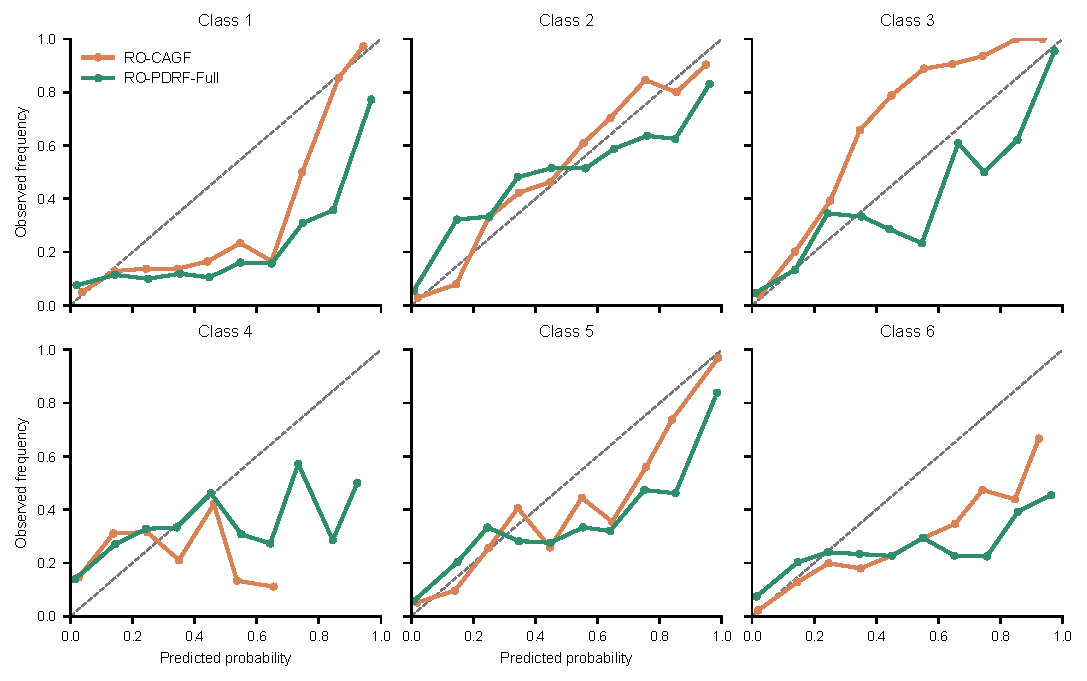
\includegraphics[width=\textwidth]{figureS5_classwise_reliability.pdf}
\caption{\textbf{Affected-row classwise calibration.} One-versus-rest predicted probability and observed class frequency for the two recovery-objective-matched ensembles. Points are shown only for non-empty bins.}
\label{fig:supp-classwise-reliability}
\end{figure}

Linear-layer operations are counted with a one-observation forward pass. Two floating-point operations are assigned per multiply--accumulate. State memory assumes 32-bit parameters; forward activation memory sums linear-layer outputs and is a reproducible footprint measure, not a device-specific peak-resident-memory claim.

\begin{table}[ht]
\centering
\caption{Inference complexity as the number of sensor groups increases.}
\resizebox{0.86\textwidth}{!}{\begin{tabular}{lrrrrr}
\toprule
Method & Groups & Parameters & FLOPs & State (KiB) & Activations (KiB) \\
\midrule
CAGF & 2 & 13326 & 26112 & 52.1 & 1.1 \\
PDRF & 2 & 9870 & 19264 & 38.6 & 0.9 \\
CAGF & 4 & 26588 & 52224 & 103.9 & 1.9 \\
PDRF & 4 & 19740 & 38528 & 77.1 & 1.9 \\
CAGF & 8 & 53112 & 104448 & 207.5 & 3.5 \\
PDRF & 8 & 39480 & 77056 & 154.2 & 3.7 \\
CAGF & 16 & 106160 & 208896 & 414.7 & 6.7 \\
PDRF & 16 & 78960 & 154112 & 308.4 & 7.4 \\
\bottomrule
\end{tabular}}
\end{table}

\begin{table}[ht]
\centering
\caption{Training stability for clean-distillation controls. Gradient norms are measured before clipping at 5.}
\resizebox{0.84\textwidth}{!}{\begin{tabular}{lrrrr}
\toprule
Method & Max epochs & Median gradient norm & Maximum gradient norm & Final selection CE \\
\midrule
CAGF+CD & 26 & 0.458 & 0.766 & 0.587 \\
EF-PD+CD & 32 & 0.425 & 1.105 & 0.382 \\
ModDrop-SD & 17 & 0.422 & 1.014 & 0.718 \\
PDRF+CD & 41 & 0.373 & 0.540 & 0.457 \\
PDRF+CD-T07 & 41 & 0.374 & 0.535 & 0.466 \\
UF-PD+CD & 46 & 0.212 & 0.353 & 0.456 \\
\bottomrule
\end{tabular}}
\end{table}

\begin{figure}[p]
\centering
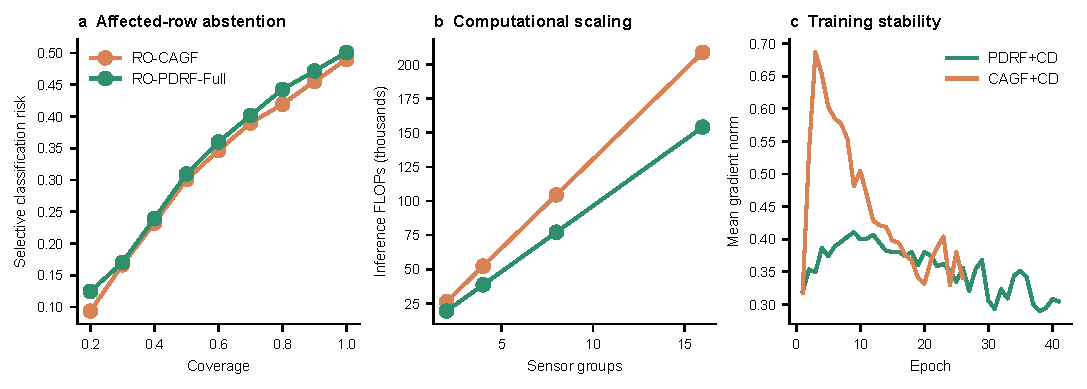
\includegraphics[width=\textwidth]{figureS6_deployment_and_complexity.pdf}
\caption{\textbf{Deployment and optimization audits.} \textbf{a}, affected-row selective classification risk. \textbf{b}, counted inference FLOPs versus sensor-group count. \textbf{c}, mean pre-clipping gradient norm by epoch for the two clean-distillation controls.}
\label{fig:supp-deployment-complexity}
\end{figure}
\FloatBarrier

\section{Archived original-protocol analyses}

The following tables and figures were generated under the original formal recovery/calibration protocol. They are retained for transparency and mechanism sensitivity, but they do not define headline method performance. Their fixed affected subset differs from the superseded seed-85000 factorial rerun; the unified headline protocol restores seed 70001 and changes the formal teacher to clean-only.

\begin{table}[ht]
\centering
\caption{Original formal-run comparator results under the fixed chemical-array silent fault.}
\resizebox{\textwidth}{!}{\begin{tabular}{llrrrrr}
\toprule
Fault & Method & Accuracy & Macro-F1 & Macro-AUPRC & Macro-AUROC & NLL\\
\midrule
natural & EF\_PD & 0.585 & 0.579 & 0.632 & 0.851 & 1.730\\
natural & UF\_PD & 0.575 & 0.561 & 0.612 & 0.856 & 1.650\\
natural & CAGF & 0.535 & 0.509 & 0.569 & 0.834 & 1.670\\
natural & DWR & 0.536 & 0.511 & 0.570 & 0.834 & 1.703\\
natural & PDRF\_NOQ & 0.590 & 0.566 & 0.642 & 0.866 & 1.793\\
natural & PDRF & 0.594 & 0.568 & 0.644 & 0.867 & 1.849\\
\addlinespace
silent & EF\_PD & 0.524 & 0.518 & 0.549 & 0.805 & 2.418\\
silent & UF\_PD & 0.527 & 0.518 & 0.549 & 0.814 & 2.251\\
silent & CAGF & 0.516 & 0.493 & 0.542 & 0.817 & 1.828\\
silent & DWR & 0.515 & 0.494 & 0.538 & 0.815 & 1.899\\
silent & PDRF\_NOQ & 0.548 & 0.533 & 0.583 & 0.835 & 2.233\\
silent & PDRF & 0.550 & 0.535 & 0.580 & 0.834 & 2.345\\
\addlinespace
\bottomrule
\end{tabular}
}
\end{table}

\begin{table}[ht]
\centering
\caption{Original formal-run mechanism ablation.}
\resizebox{0.78\textwidth}{!}{\begin{tabular}{lrrrr}
\toprule
Variant & Accuracy & Macro-AUPRC & Macro-AUROC & NLL\\
\midrule
PD\_ONLY & 0.531 & 0.556 & 0.817 & 2.138\\
PD\_MONO & 0.537 & 0.563 & 0.821 & 2.071\\
PD\_RANK & 0.514 & 0.547 & 0.812 & 2.309\\
NO\_LSCORE & 0.514 & 0.545 & 0.811 & 2.312\\
LSCORE\_NO\_LRANK & 0.547 & 0.555 & 0.822 & 2.441\\
PDRF & 0.550 & 0.580 & 0.834 & 2.345\\
\bottomrule
\end{tabular}
}
\end{table}

\begin{table}[ht]
\centering
\caption{Original formal-run recovery and calibration results. Aff. denotes the affected subset.}
\resizebox{\textwidth}{!}{\begin{tabular}{lrrrrrrrr}
\toprule
Method & All Acc. & All AUROC & Aff. Acc. & Aff. F1 & Aff. AUPRC & Aff. AUROC & Aff. NLL & Aff. ECE \\
\midrule
CAGF & 0.516 & 0.817 & 0.474 & 0.454 & 0.505 & 0.792 & 2.095 & 0.277 \\
PDRF & 0.550 & 0.834 & 0.476 & 0.471 & 0.509 & 0.791 & 3.085 & 0.369 \\
RO-PDRF-Full & 0.558 & 0.840 & 0.493 & 0.483 & 0.527 & 0.804 & 2.693 & 0.344 \\
\bottomrule
\end{tabular}}
\end{table}

\begin{figure}[p]
\centering
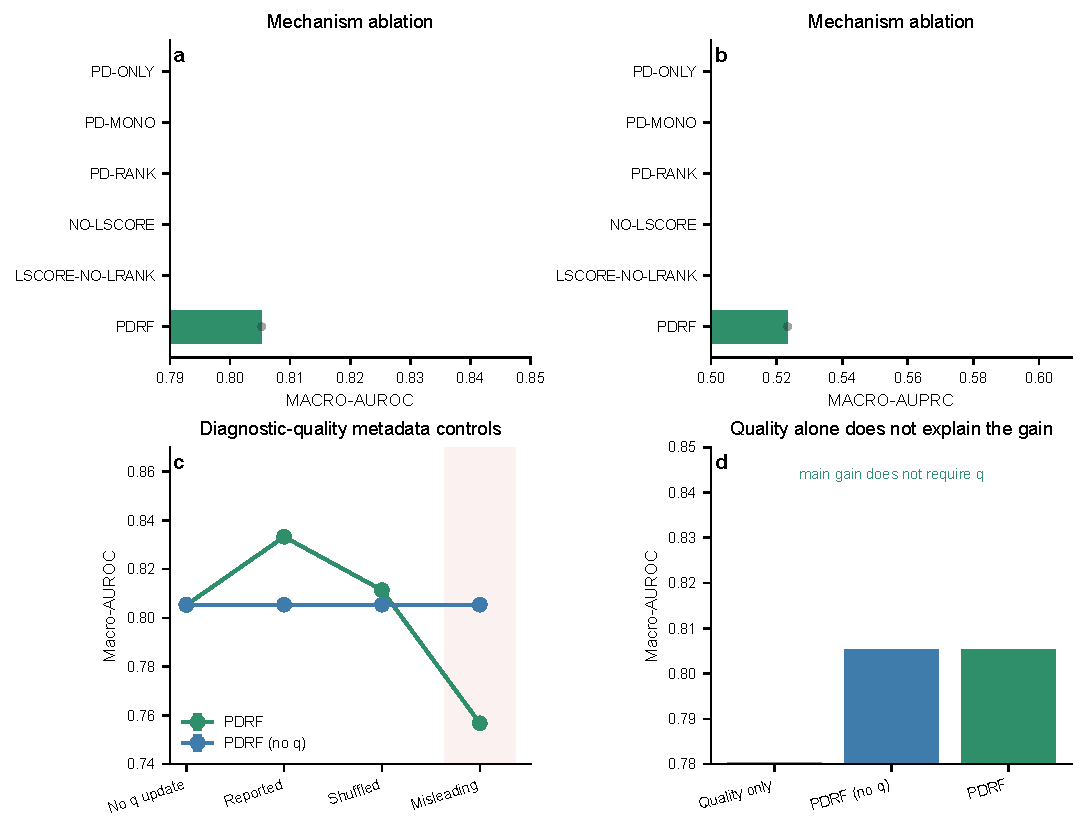
\includegraphics[width=\textwidth]{figure4_mechanism_quality.pdf}
\caption{\textbf{Original-protocol mechanism and diagnostic-quality controls.} Mechanism ablations, metadata perturbations and a quality-only comparator are retained as sensitivity evidence.}
\end{figure}

\begin{figure}[p]
\centering
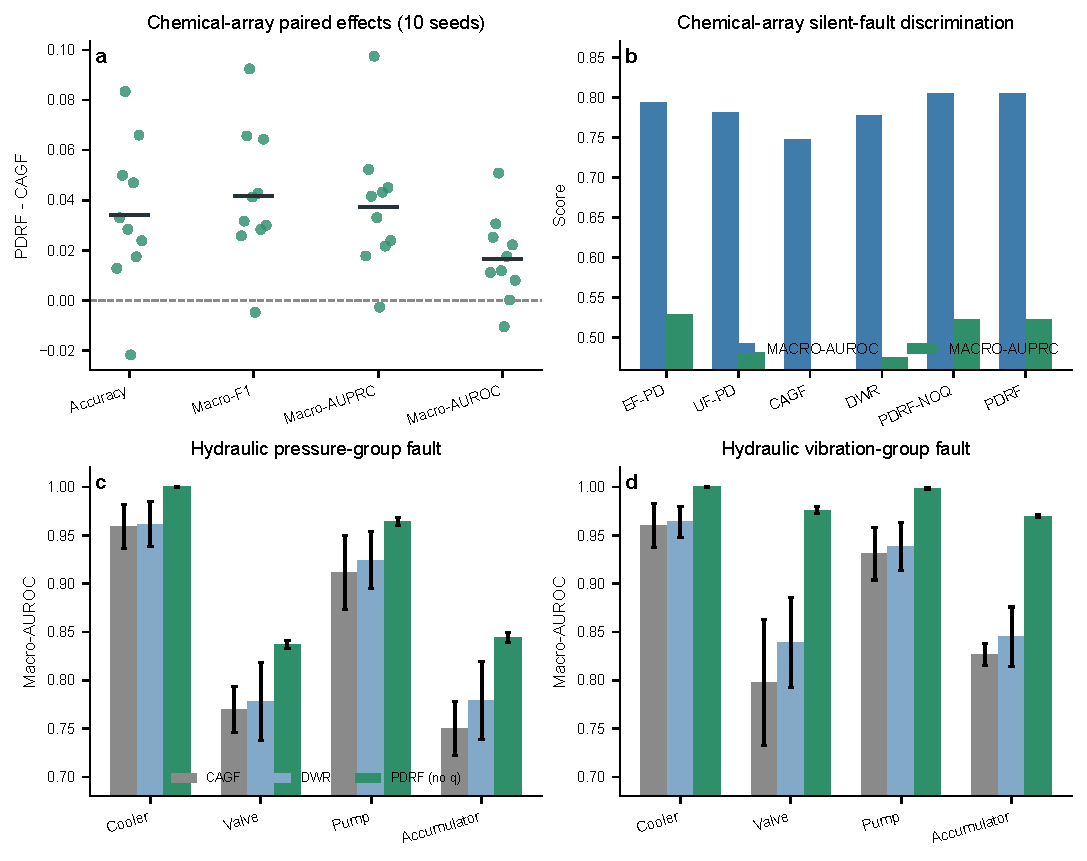
\includegraphics[width=\textwidth]{figure3_main_results.pdf}
\caption{\textbf{Original-protocol controlled-fault comparisons.} Chemical seed-level effects and hydraulic task results are retained for protocol transparency; the clean-teacher recovery-objective-matched figure supplies the headline comparison.}
\end{figure}

\begin{figure}[p]
\centering
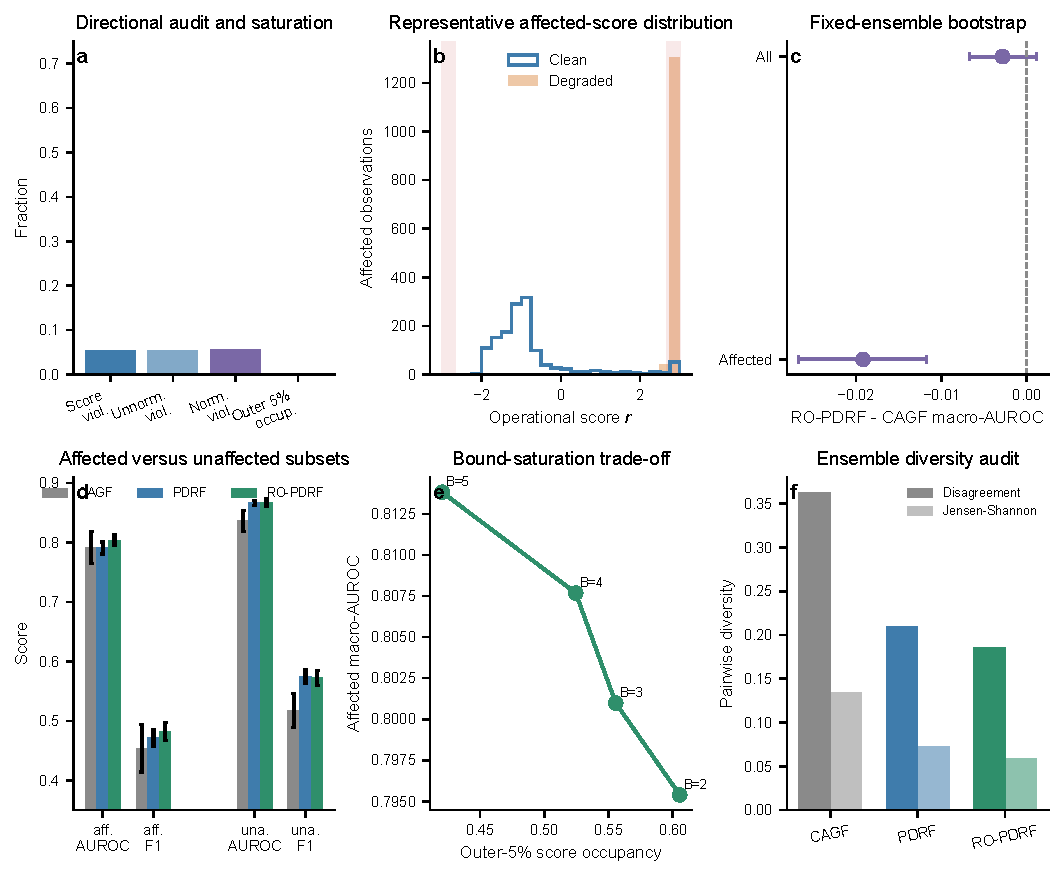
\includegraphics[width=\textwidth]{figure5_boundaries_remedies.pdf}
\caption{\textbf{Boundary analyses and recovery audits.} Directional violations, bounded-response saturation, fixed-ensemble bootstrap effects, affected/unaffected outcomes, bound sensitivity and ensemble diversity. This dense diagnostic figure is moved from the main paper to preserve the complete evidence without overloading the principal narrative.}
\label{fig:supp-boundaries}
\end{figure}

\begin{figure}[p]
\centering
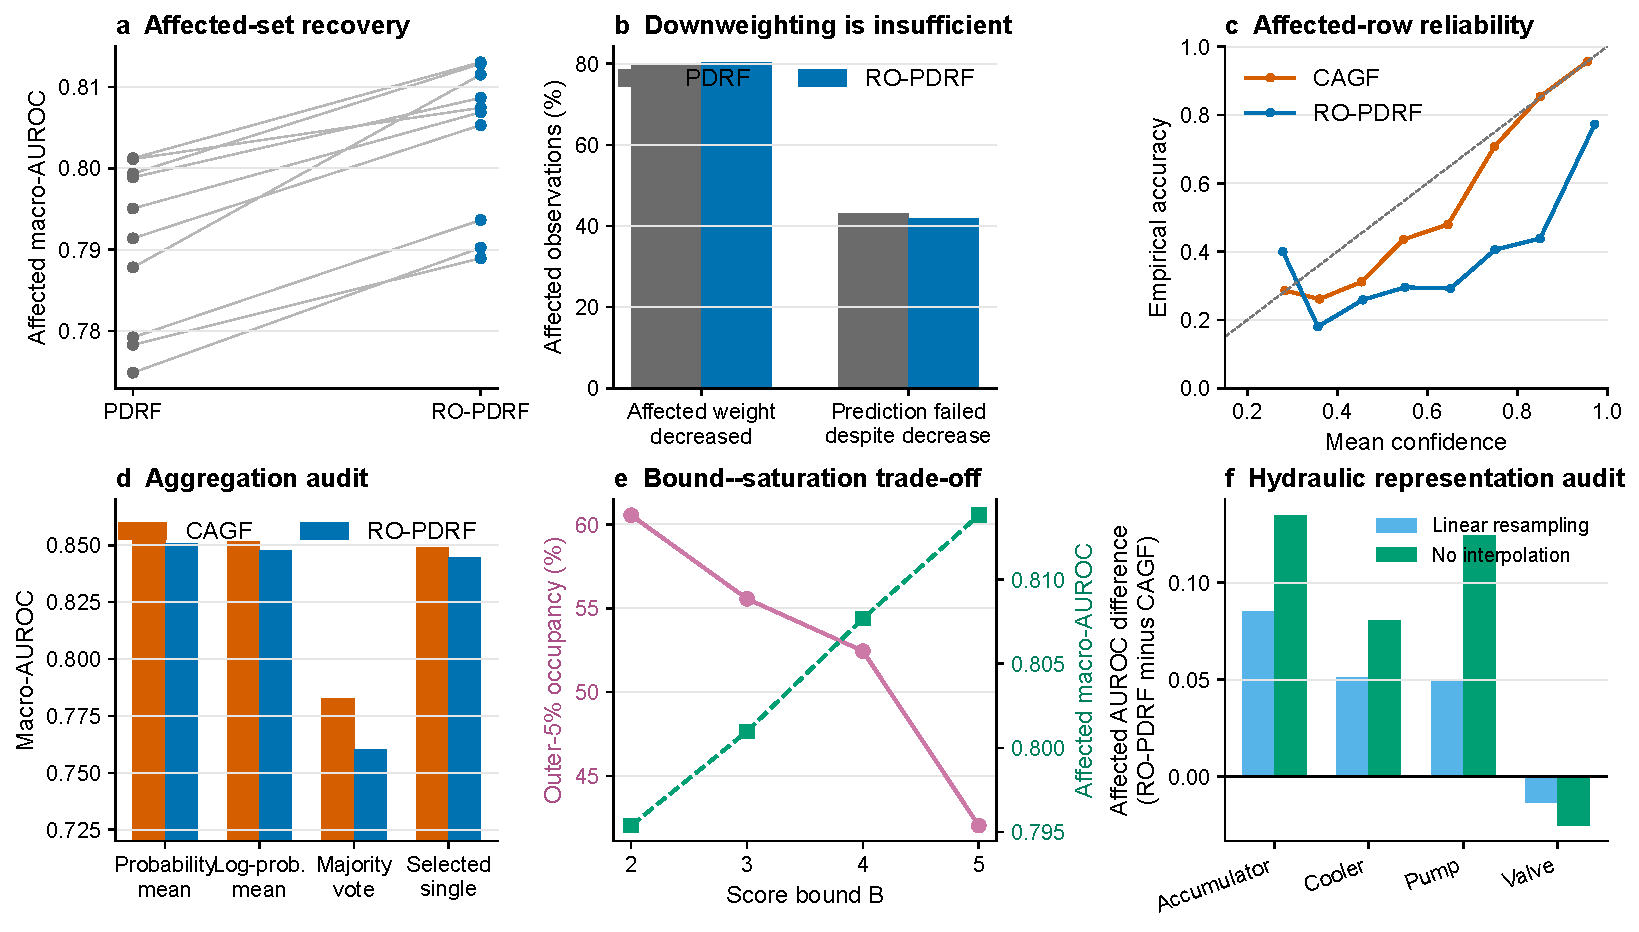
\includegraphics[width=\textwidth]{figure6_recovery_mechanism.pdf}
\caption{\textbf{Prediction-level recovery and deployment audits.} Matched recovery, failures despite downweighting, affected-row calibration, aggregation rules, score-bound sensitivity and hydraulic representation robustness.}
\label{fig:supp-recovery}
\end{figure}
\FloatBarrier

\section{External public-data feasibility audit}

We searched for an external dataset that simultaneously provides (i) naturally occurring or maintenance-confirmed sensor failure, (ii) an independent downstream state to recover after suppressing the faulty sensor and (iii) multiple physical devices or sites. The NASA sensor-fault resource (\url{https://data.nasa.gov/dataset/modeling-detection-and-disambiguation-of-sensor-faults-for-aerospace-applications}) describes experimental actuator data and simulated sensor faults, but its public landing page does not provide a directly usable natural sensor-failure cohort with an independent recovery target. BASiC (\url{https://doi.org/10.5281/zenodo.8195068}) contains 70 autonomous aerial-vehicle flights, but its failures are introduced through software-in-the-loop rather than documented natural hardware sensor failures. ALFA (\url{https://theairlab.org/alfa-dataset/}) contains real flight records with engine and control-surface failures, which are actuator or system failures rather than the required sensor-failure annotation. The AHU data used here contain operational sensor-fault labels but no independent downstream recovery target; the hydraulic data contain native component targets but controlled sensor interventions and one rig. We therefore did not relabel actuator failures as sensor faults or construct a circular downstream target. The absence of a qualifying public dataset remains a limitation rather than evidence of external field recovery.

\section{Reproducibility and scope}

The Q1 entry points are \path{run_cee_lite_routing_validation.py}, \path{analyse_cee_lite_results.py}, \path{analyse_cee_q1_scores.py}, \path{analyse_cee_fault_plausibility.py}, \path{run_cee_strict88_additional_audits.py}, \path{analyse_cee_strict88_revision.py} and \path{make_cee_q1_figures.py}. The machine-readable frozen design is \path{cee_cf10_r2_lite_config.json}; the added audit design is \path{source_data/strict88_additional_audits_design.json}. Exact local package versions are recorded in \path{requirements-lock.txt} and \path{environment.yml}. Prediction-level outputs, selector thresholds, safety accounting, model costs, probability metrics, fixed-mechanism/batch intervals, deployment-support decisions, mild-severity results and fixed-thread timings are stored under \path{source_data/q1_*} and \path{source_data/strict88_*}. The routing API emits the selected probability vector by default and, when requested, also returns endpoint identity and the conditional preference score. Figures use Python/matplotlib exclusively. Editable SVG/PDF figures and 600-dpi TIFFs are included. The submitted Supplementary Information retains all legacy selector baselines, fault-severity grids, calibration-size analyses, fitted coefficients and the script-to-result manifest so that negative and superseded analyses remain auditable. The versioned release archive contains a SHA-256 manifest, and the public repository URL and exact commit are reported in the main article.

The chemical-array experiment uses real longitudinal measurements with controlled feature-level sensor faults. The hydraulic experiment uses native test-rig component-condition labels with controlled sensor faults. The AHU audit adds naturally observed operational records with expert-annotated sensor-fault classes from 41 installed AHUs across three buildings. Those labels were assigned from engineering rules and expert review rather than maintenance-confirmed sensor replacement records. The evidence supports a controlled-corruption risk-control protocol and a field-operational direct-diagnosis boundary, not hardware-failure prognosis, downstream field recovery or zero-shot building transfer.

\end{document}
